% Generated by scripts/review.py sync. Layout sources are shared; edit a copied command.
% Generated by scripts/review.py sync; edit templates/studio sources.
\documentclass[aspectratio=169]{beamer}
\usetheme{bitpolito-studio}
\usepackage{bitpolitostudiotemplates}
\usepackage[backend=biber]{biblatex}
\addbibresource{bibliography.bib}
\title{Studio\\Layout Library}
\author{BitPolito}
\institute{Editable slide templates}
\date{}
\begin{document}
\section{Opening}
\gdef\studiocataloguename{\detokenize{cover}}
\studiotemplate[
  variant={pattern},
  palette={blue},
  text/1={First Last},
  text/2={Bitcoin is not\\Crypto!},
  text/3={BitPolito --- Politecnico di Torino}
]{cover}
\gdef\studiocataloguename{\detokenize{contents}}
\studiotemplate[
  variant={panels},
  palette={light},
  text/3={Contents},
  text/1={Why Bitcoin?},
  text/2={Distributed systems},
  text/4={Blockchain},
  text/5={Open-source development}
]{agenda}
\gdef\studiocataloguename{\detokenize{section-divider}}
\studiotemplate[
  variant={default},
  palette={blue},
  text/1={Why Bitcoin?}
]{section-divider}
\gdef\studiocataloguename{\detokenize{tabbed-agenda}}
\studiotemplate[
  variant={rail},
  palette={light},
  text/1={Why join BitPolito}
]{agenda}
\gdef\studiocataloguename{\detokenize{cover-light}}
\studiotemplate[
  variant={wide-pattern},
  palette={light},
  text/1={Sibilla Merlo},
  text/2={Computing\\basics},
  text/3={BitGeneration --- Politecnico di Torino}
]{cover}
\gdef\studiocataloguename{\detokenize{cover-photo}}
\studiotemplate[
  variant={photo},
  palette={light},
  text/1={Gianluca Cappiello},
  text/2={Cryptography},
  text/3={BitGeneration --- Politecnico di Torino}
]{cover}
\gdef\studiocataloguename{\detokenize{cover-script-blue}}
\studiotemplate[
  variant={script},
  palette={light},
  text/3={XDVJAVXXDVHJPIVOM\\VINVUDJIZWDOXJDI},
  text/1={Shall we make\\a Bitcoin\\transaction?},
  text/2={Shall we make\\a Bitcoin\\transaction?}
]{cover}
\gdef\studiocataloguename{\detokenize{cover-dashboard}}
\studiotemplate[
  variant={default},
  palette={blue},
  text/5={8,000+},
  text/6={Followers across channels},
  text/7={60+},
  text/8={Events organized},
  text/9={G. Cappiello --- BKCH26},
  text/1={55},
  text/3={Participants},
  text/2={210},
  text/4={Alumni}
]{cover-dashboard}
\gdef\studiocataloguename{\detokenize{cover-wide-title}}
\studiotemplate[
  variant={wide-title},
  palette={blue},
  text/2={Lightning Network},
  text/3={Massimo Musumeci},
  text/1={2024}
]{cover}
\gdef\studiocataloguename{\detokenize{agenda-with-icons}}
\studiotemplate[
  variant={icons},
  palette={light},
  text/1={BitPolito's offer}
]{agenda}
\gdef\studiocataloguename{\detokenize{agenda-with-schedule}}
\studiotemplate[
  variant={schedule},
  palette={light},
  text/3={Meetings},
  text/5={Every Thursday},
  text/4={Once per month},
  text/1={Everyday},
  text/2={Twice per month}
]{agenda}
\section{Statements}
\gdef\studiocataloguename{\detokenize{statement-arrow}}
\studiotemplate[
  variant={arrow},
  palette={light},
  text/1={The economic and\\monetary system is in crisis}
]{statement}
\gdef\studiocataloguename{\detokenize{glow-statement}}
\studiotemplate[
  variant={glow},
  palette={light},
  text/1={Bridging university and\\Bitcoin industry}
]{statement}
\gdef\studiocataloguename{\detokenize{blue-statement}}
\studiotemplate[
  variant={plain},
  palette={blue},
  text/1={Every UTXO needs a signature to be spent}
]{statement}
\gdef\studiocataloguename{\detokenize{icon-spotlight-light}}
\studiotemplate[
  variant={compact},
  palette={light},
  text/1={Passion becomes\\the mission}
]{icon-spotlight}
\gdef\studiocataloguename{\detokenize{icon-spotlight-blue}}
\studiotemplate[
  variant={large},
  palette={blue},
  text/1={Absolutely scarce\\digital commodity}
]{icon-spotlight}
\gdef\studiocataloguename{\detokenize{oversized-word}}
\studiotemplate[
  variant={clipped},
  palette={light},
  text/2={Discovery},
  text/1={Bitcoin is}
]{statement}
\gdef\studiocataloguename{\detokenize{chat-dialogue}}
\studiotemplate[
  variant={two-messages},
  palette={blue},
  text/1={"A private matter is something one does not\\want the whole world to know, while a secret\\matter is something one does not want anyone\\to know. Privacy is the power to selectively\\reveal oneself to the world."},
  text/2={--- Eric Hughes, A Cypherpunk''s Manifesto, 1993}
]{dialogue}
\gdef\studiocataloguename{\detokenize{speech-panel}}
\studiotemplate[
  variant={people},
  palette={light},
  text/1={Let's talk about Bitcoin in our university!\\Of course only technical stuff...},
  text/2={February 2020}
]{dialogue}
\gdef\studiocataloguename{\detokenize{chat-three-messages}}
\studiotemplate[
  variant={three-messages},
  palette={light},
  text/1={Hurry up, you are going to be the next\\enlightened ruling class!},
  text/3={It's not needed.},
  text/2={But you had never explained me how\\the society works and what are the\\values behind it...}
]{dialogue}
\gdef\studiocataloguename{\detokenize{oversized-number-light}}
\studiotemplate[
  variant={plain},
  palette={blue}
]{oversized-number}
\gdef\studiocataloguename{\detokenize{oversized-number-blue}}
\studiotemplate[
  variant={captioned},
  palette={blue},
  text/1={Renewable energy},
  text/2={Source: Bitcoin Mining Council}
]{oversized-number}
\gdef\studiocataloguename{\detokenize{diagonal-photo-title}}
\studiotemplate[
  variant={diagonal},
  palette={light},
  text/1={10\textsuperscript{\fontsize{270\studiounit}{310\studiounit}\selectfont77} keys}
]{image-text}
\gdef\studiocataloguename{\detokenize{title-paragraphs}}
\studiotemplate[
  variant={left},
  palette={light},
  text/1={General LNURL features},
  text/3={A range of accepted amounts can be specified.},
  text/4={Additional metadata: longer descriptions, images and messages.},
  text/6={No expiry time.},
  text/5={Static: reusable, so it can be printed or displayed permanently\\on a website.},
  text/2={Asynchronous.}
]{paragraphs}
\gdef\studiocataloguename{\detokenize{title-centered-paragraphs}}
\studiotemplate[
  variant={centered},
  palette={light},
  text/1={Bolt-12},
  text/2={BOLT12 offers a similar service without a web server, with improved\\privacy. It is native to Lightning.},
  text/4={LNURL is widely adopted and field-tested. It can suit shops and\\businesses that already operate web servers.},
  text/3={BUT}
]{paragraphs}
\gdef\studiocataloguename{\detokenize{statement-with-credit}}
\studiotemplate[
  variant={credit},
  palette={light},
  text/1={The scale of numbers},
  text/4={10\textsuperscript{12} s},
  text/2={30,000 BCE},
  text/6={32 years ago},
  text/3={11 days ago},
  text/5={10\textsuperscript{9} s}
]{statement}
\gdef\studiocataloguename{\detokenize{people-speech-cards}}
\studiotemplate[
  variant={cards},
  palette={light},
  text/1={Linux is\\a cancer},
  text/2={Open source is\\un-American},
  text/3={Free software\\is communism},
  text/4={Ballmer},
  text/5={Allchin},
  text/6={Gates},
  text/7={GNU and Linux scared entrenched powers, but just\\worked better and developed a global community}
]{dialogue}
\gdef\studiocataloguename{\detokenize{paired-icons-blue}}
\studiotemplate[
  variant={default},
  palette={blue}
]{paired-icons-blue}
\section{Lists}
\gdef\studiocataloguename{\detokenize{two-columns}}
\studiotemplate[
  variant={default},
  palette={light},
  text/1={Different approaches},
  text/5={Asynchronous transactions\par UTXOs, coin selection and\\transaction construction\par Send and receive funds\par Fee models and waiting times\par Record transactions in blocks\\and consider privacy\par Passive chain analysis\\for information gathering},
  text/6={Synchronous transactions\par Receiving funds requires\\inbound liquidity\par Channels, liquidity and\\balancing\par Routing, fees and waiting times\par Privacy considerations\par Active information gathering},
  text/3={Bitcoin Base Layer},
  text/4={Layer 2: Lightning},
  text/2={Lightning enables even very small payments, transferred instantly\\with minimal fees.}
]{two-columns}
\gdef\studiocataloguename{\detokenize{list-rail-light}}
\studiotemplate[
  variant={three-items},
  palette={light},
  text/2={Distributed\\systems},
  text/1={No central coordinator},
  text/3={Common rules},
  text/4={Client-server symmetry}
]{list-rail}
\gdef\studiocataloguename{\detokenize{list-rail-blue}}
\studiotemplate[
  variant={four-items},
  palette={blue},
  text/3={The Bitcoin system is},
  text/1={Trustless},
  text/2={Decentralized},
  text/4={Immutable},
  text/5={Transparent}
]{list-rail}
\gdef\studiocataloguename{\detokenize{grouped-rail}}
\studiotemplate[
  variant={grouped},
  palette={light},
  text/4={Fiat money},
  text/1={Money creation},
  text/2={Central bank},
  text/3={Commercial banks},
  text/5={Consequences},
  text/6={Cantillon effect},
  text/7={Lost purchasing power}
]{list-rail}
\gdef\studiocataloguename{\detokenize{labelled-rows}}
\studiotemplate[
  variant={default},
  palette={light},
  text/1={The change},
  text/4={The comparison},
  text/6={Who comes later},
  text/2={A friend changes only their own notebook},
  text/5={Others see that it does not match\\and discard it.},
  text/7={Copy and check from page one:\\do not trust, verify.},
  text/3={What if\\someone cheats?}
]{labelled-rows}
\gdef\studiocataloguename{\detokenize{checklist-rail}}
\studiotemplate[
  variant={default},
  palette={blue},
  text/3={Installing\\RaspiBlitz},
  text/1={\textbf{Download the RaspiBlitz image}\\{\fontsize{36\studiounit}{43\studiounit}\selectfont From the official GitHub repository or website.}},
  text/2={\textbf{Write the image to an SD card}\\{\fontsize{36\studiounit}{43\studiounit}\selectfont Use balenaEtcher to write it to a microSD card.}},
  text/4={\textbf{Configure the device}\\{\fontsize{36\studiounit}{43\studiounit}\selectfont Insert the SD card and SSD into the Raspberry Pi.}},
  text/5={\textbf{Start RaspiBlitz}\\{\fontsize{36\studiounit}{43\studiounit}\selectfont Connect network and power; use a monitor\\to follow the installation.}}
]{checklist-rail}
\gdef\studiocataloguename{\detokenize{feature-spotlight}}
\studiotemplate[
  variant={default},
  palette={light},
  text/3={Scaling a protocol},
  text/4={A system can handle more\\data or users without\\compromising performance\\or stability.},
  text/5={Handle more transactions\\per second with lower\\fees, while preserving\\security and\\decentralization.},
  text/6={Bitcoin},
  text/1={Handle more simultaneous\\connections, increase\\data transmission speed\\or provide greater\\processing capacity.},
  text/2={Internet}
]{feature-spotlight}
\gdef\studiocataloguename{\detokenize{privacy-levels}}
\studiotemplate[
  variant={default},
  palette={light},
  text/2={Privacy\\levels},
  text/4={No-KYC: no personal information\\is requested},
  text/3={Soft-KYC: a minimum of personal\\information is requested},
  text/1={Full-KYC: identity verification\\by submitting documents}
]{levels}
\gdef\studiocataloguename{\detokenize{title-two-column-list}}
\studiotemplate[
  variant={default},
  palette={light},
  text/1={Summary},
  text/2={\textbullet{} Bitcoin on-chain: base layer and\\layer 2\par\hangindent=1em\textbullet{} Different ideas, timing, fee models\\and scalability\par\hangindent=1em\textbullet{} Why Lightning suits everyday\\payments\par\hangindent=1em\textbullet{} Nodes, channels, liquidity\\and balancing\par\hangindent=1em\textbullet{} Asynchronous on-chain versus\\synchronous Lightning\par\hangindent=1em\textbullet{} Routing},
  text/3={\textbullet{} Explore a Lightning node\par\hangindent=1em\textbullet{} Privacy differences\par\hangindent=1em\textbullet{} Self-custodial nodes on local\\hardware or in the cloud\par\hangindent=1em\textbullet{} Lightning service providers\par\hangindent=1em\textbullet{} On-demand nodes\par\hangindent=1em\textbullet{} Custodial and self-custodial\\wallets and LNDHub interfaces\par\hangindent=1em\textbullet{} BOLT11 and LNURL\par\hangindent=1em\textbullet{} Payment processors\par\hangindent=1em\textbullet{} Implementations: Core Lightning, LND}
]{title-two-column-list}
\gdef\studiocataloguename{\detokenize{partner-rail}}
\studiotemplate[
  variant={default},
  palette={light},
  text/1={bitbox.swiss},
  text/2={@BitBoxSwiss},
  text/10={fulgur.ventures},
  text/11={@fulgurventures},
  text/3={planb.lugano.ch},
  text/4={@LuganoPlanB},
  text/5={bitrefill.com},
  text/7={@bitrefill},
  text/8={zebedee.io},
  text/9={@zbdapp},
  text/6={Partner\&Sponsor},
  graphic/2={
\includegraphics{images/studio/collection/figma-0996-part-01.pdf}},
  graphic/4={
\includegraphics{images/studio/collection/figma-0996-part-02.pdf}},
  graphic/3={
\includegraphics{images/studio/collection/figma-0996-part-03.pdf}},
  graphic/14={
\includegraphics{images/studio/collection/figma-0996-part-04.pdf}},
  graphic/16={
\includegraphics{images/studio/collection/figma-0996-part-05.pdf}},
  graphic/15={
\includegraphics{images/studio/collection/figma-0996-part-06.pdf}},
  graphic/1={
\includegraphics{images/studio/collection/figma-0996-part-07.pdf}},
  graphic/7={
\includegraphics{images/studio/collection/figma-0996-part-08.pdf}},
  graphic/6={
\includegraphics{images/studio/collection/figma-0996-part-09.pdf}},
  graphic/5={
\includegraphics{images/studio/collection/figma-0996-part-10.pdf}},
  graphic/10={
\includegraphics{images/studio/collection/figma-0996-part-11.pdf}},
  graphic/9={
\includegraphics{images/studio/collection/figma-0996-part-12.pdf}},
  graphic/8={
\includegraphics{images/studio/collection/figma-0996-part-13.pdf}},
  graphic/13={
\includegraphics{images/studio/collection/figma-0996-part-14.pdf}},
  graphic/12={
\includegraphics{images/studio/collection/figma-0996-part-15.pdf}},
  graphic/11={
\includegraphics{images/studio/collection/figma-0996-part-16.pdf}}
]{partner-rail}
\gdef\studiocataloguename{\detokenize{icon-rail}}
\studiotemplate[
  variant={default},
  palette={light},
  text/4={Graphic Designer},
  text/2={Video Maker},
  text/1={Video Editor},
  text/3={Marketing}
]{icon-rail}
\gdef\studiocataloguename{\detokenize{privacy-levels-blue}}
\studiotemplate[
  variant={default},
  palette={blue},
  text/2={Privacy\\levels},
  text/4={No-KYC: no personal information\\is requested},
  text/3={Soft-KYC: a minimum of personal\\information is requested},
  text/1={Full-KYC: identity verification\\by submitting documents}
]{levels}
\gdef\studiocataloguename{\detokenize{stepped-rail-blue}}
\studiotemplate[
  variant={stepped},
  palette={blue},
  text/2={Installing\\RaspiBlitz},
  text/5={Hardware needed},
  text/1={Raspberry Pi 4\\{\fontsize{40\studiounit}{46\studiounit}\selectfont 4GB or 8GB preferred}},
  text/6={Power supply and cables,\\with an optional display\\for monitoring},
  text/3={External SSD},
  text/4={1TB recommended}
]{list-rail}
\section{Cards}
\gdef\studiocataloguename{\detokenize{three-cards}}
\studiotemplate[
  variant={three},
  palette={light},
  text/1={Financial exclusion},
  text/2={Unbanked},
  text/3={Remittances},
  text/4={Censorship}
]{icon-cards}
\gdef\studiocataloguename{\detokenize{three-step-process}}
\studiotemplate[
  variant={three},
  palette={light},
  text/2={360\textdegree{} education},
  text/3={In-depth study},
  text/1={Global overview}
]{icon-process}
\gdef\studiocataloguename{\detokenize{two-cards}}
\studiotemplate[
  variant={two},
  palette={light},
  text/2={Security},
  text/1={Privacy}
]{icon-cards}
\gdef\studiocataloguename{\detokenize{four-card-grid}}
\studiotemplate[
  variant={four},
  palette={light},
  text/1={How Bitcoin works},
  text/2={{\fontsize{75.16\studiounit}{87.1856\studiounit}\selectfont Proof of Work (What)}\\\textbullet{} Scarcity vs. privacy\\\textbullet{} Hashes and difficulty adjustment},
  text/4={Timechain (When)},
  text/6={\textbullet{} Durability/Scarcity},
  text/3={{\fontsize{75.16\studiounit}{87.1856\studiounit}\selectfont Proof of Knowledge (Who)}\\\textbullet{} Privacy vs. scarcity\\\textbullet{} Asymmetric cryptography},
  text/5={{\fontsize{75.16\studiounit}{87.1856\studiounit}\selectfont Lightning Network (Where)}\\\textbullet{} Scalability/Privacy}
]{text-cards}
\gdef\studiocataloguename{\detokenize{eight-icon-grid}}
\studiotemplate[
  variant={eight},
  palette={light},
  text/1={Education},
  text/4={Marketing},
  text/5={Design},
  text/2={Events},
  text/7={Management},
  text/6={Cryptography},
  text/3={Divisions}
]{icon-grid}
\gdef\studiocataloguename{\detokenize{four-step-process}}
\studiotemplate[
  variant={four},
  palette={light},
  text/1={Student's journey},
  text/2={Understand\\Bitcoin's potential},
  text/3={Attend\\education path},
  text/5={Get a job in\\Bitcoin industry},
  text/4={Acquire new\\competences}
]{icon-process}
\gdef\studiocataloguename{\detokenize{two-step-process}}
\studiotemplate[
  variant={two},
  palette={light},
  text/2={Technology},
  text/1={Values}
]{icon-process}
\gdef\studiocataloguename{\detokenize{milestone-cards}}
\studiotemplate[
  variant={milestones},
  palette={light},
  text/1={Plan B Forum\\El Salvador},
  text/2={Barcelona\\Cypher\\Conference},
  text/3={BitCuneo},
  text/4={BitCare Forum},
  text/5={BTC Prague},
  text/6={Missions}
]{icon-process}
\gdef\studiocataloguename{\detokenize{twelve-word-grid}}
\studiotemplate[
  variant={twelve},
  palette={light},
  text/1={Private key},
  text/2={1. issue},
  text/5={4. lyrics},
  text/8={7. announce},
  text/10={10. damage},
  text/3={2. flame},
  text/6={5. find},
  text/9={8. banner},
  text/11={11. civil},
  text/4={3.sample},
  text/7={6. vault},
  text/12={12. goat}
]{icon-grid}
\gdef\studiocataloguename{\detokenize{three-card-summary}}
\studiotemplate[
  variant={summary},
  palette={light},
  text/1={Key concepts recap},
  text/2={Decentralization},
  text/4={A foundation of Bitcoin: provides\\security and censorship resistance.},
  text/3={The role of nodes},
  text/5={Independent validation: each node checks\\the protocol rules; the timechain preserves\\a history of transactions.},
  text/6={Workshop goal},
  text/7={Explore options for running a node;\\provide practical steps to get started.}
]{icon-cards}
\gdef\studiocataloguename{\detokenize{four-pillar-cards}}
\studiotemplate[
  variant={four-pillars},
  palette={light},
  text/1={Bitcoin consensus},
  text/2={Shared rules},
  text/4={Nodes enforce the same rules, ensuring\\consistency across the network.},
  text/3={Example},
  text/5={Every new block may create only a\\limited number of new bitcoin.},
  text/6={Outside consensus},
  text/8={Some protocol rules fall outside network\\consensus, such as the algorithm used\\to gossip messages.},
  text/7={Changing consensus},
  text/9={Soft fork: add new consensus rules.\\Hard fork: remove consensus rules.}
]{icon-cards}
\gdef\studiocataloguename{\detokenize{hardware-options}}
\studiotemplate[
  variant={devices},
  palette={blue},
  text/2={Casa Node},
  text/6={Nodl},
  text/1={Preconfigured devices},
  text/3={Features:\\Lightning Network\\integration\\User-friendly interface},
  text/7={Features:\\Advanced services\\such as BTCPay Server\\Advanced privacy options},
  text/5={Indicative price:\\About \$300-\$400},
  text/8={Indicative price:\\Starting at \$500},
  text/4={Hardware\\solutions}
]{options}
\gdef\studiocataloguename{\detokenize{software-options}}
\studiotemplate[
  variant={applications},
  palette={light},
  text/1={Umbrel},
  text/5={MyNode},
  text/2={Features:\\An intuitive interface\\An app store for extending\\functionality},
  text/3={Installation:\\Download the image to a\\bootable USB drive or SD card,\\then follow the installation\\wizard on the dedicated\\hardware.},
  text/6={Features:\\Free version with basic functions\\Premium version with additional\\features},
  text/7={Installazione:\\\textbullet{} Richiede alcuni passaggi\\manuali, ma offre maggiore\\controllo sull'hardware dedicato},
  text/4={Available\\software}
]{options}
\gdef\studiocataloguename{\detokenize{two-card-vertical}}
\studiotemplate[
  variant={two-vertical},
  palette={light},
  text/1={Upper layers\\\textbullet{} Rapid innovation\\\textbullet{} Protocol competition},
  text/4={Lower layers\\\textbullet{} Stability\\\textbullet{} Robustness\\\textbullet{} Ossification\\\textbullet{} Convergence},
  text/2={Scaling a protocol},
  text/3={Layered architectures help engineers\\build systems with greater stability\\and robustness, much like the\\structure of a building.}
]{icon-cards}
\gdef\studiocataloguename{\detokenize{callout-explanation}}
\studiotemplate[
  variant={callout},
  palette={light},
  text/1={ZK-STARKs for\\Lightning Network},
  text/2={Off-chain channels\hspace{220\studiounit}scalable payments},
  text/4={\textbullet{} Privacy = balance / route proofs},
  text/5={without revealing data},
  text/6={\textbullet{} Security = compact proofs of channel},
  text/7={state},
  text/8={\textbullet{} Challenge = Integration with LN protocols,},
  text/9={efficient verification required},
  text/3={Use STARKs to prove channel\\correctness without revealing\\balances or requiring full\\channel history}
]{text-cards}
\gdef\studiocataloguename{\detokenize{six-outline-cards}}
\studiotemplate[
  variant={six-outline},
  palette={light},
  text/1={What to consider},
  text/3={Difficulty level},
  text/5={Bitcoin price},
  text/7={Payment method},
  text/2={Energy price},
  text/4={Capital Expenditure (CapEx)},
  text/6={Geopolitics}
]{text-cards}
\gdef\studiocataloguename{\detokenize{six-explanation-cards}}
\studiotemplate[
  variant={six-detailed},
  palette={light},
  text/1={Wallet Lightning Network},
  text/3={A keystore holding secrets, such as\\private keys},
  text/5={Manages channel opening and closing},
  text/6={Finds a connected channel route from\\the payer to the payment recipient},
  text/2={A Bitcoin node stores blockchain data\\and communicates with other nodes},
  text/4={A Lightning node communicates on\\the peer-to-peer network},
  text/7={A map of announced nodes and channels}
]{text-cards}
\gdef\studiocataloguename{\detokenize{five-icon-row}}
\studiotemplate[
  variant={row},
  palette={light},
  text/1={Benefits},
  text/6={Low\\fees},
  text/3={Micropayment\\support},
  text/5={Low energy\\use},
  text/4={More\\privacy},
  text/2={Fast\\transactions}
]{icon-grid}
\gdef\studiocataloguename{\detokenize{square-icon-grid}}
\studiotemplate[
  variant={four},
  palette={light},
  text/2={Divisions},
  text/1={Education},
  text/3={Marketing},
  text/4={Management}
]{icon-grid}
\gdef\studiocataloguename{\detokenize{incentives-card-grid}}
\studiotemplate[
  variant={default},
  palette={light},
  text/1={Incentives},
  text/4={- Block reward (new BTC)\\\textbullet{} Transaction fees},
  text/2={Miner},
  text/8={Build on a neutral, open protocol},
  text/7={Developer},
  text/11={Fixed supply = protection from inflation},
  text/10={Long-term Holder},
  text/5={- Censorship-resistant\\- Permissionless payments},
  text/3={Merchant / User},
  text/9={- Sovereignty: verify your own\\transactions\par \textbullet{} Strengthen network\\decentralization},
  text/6={Full Node Operator}
]{incentives-card-grid}
\gdef\studiocataloguename{\detokenize{network-environments}}
\studiotemplate[
  variant={default},
  palette={light},
  text/1={Network Environments},
  text/2={Mainnet},
  text/4={The real Bitcoin network. Real BTC. Real value.\\No mistakes. Chain started: January 3, 2009\\Use for: production, real transactions},
  text/3={Testnet (testnet3/testnet4)},
  text/5={Public test network. Coins are worthless (tBTC).\\Anyone can mine. Difficulty fluctuates wildly.\\Use for: public integration testing, faucet coins},
  text/6={Regtest},
  text/8={Local private blockchain. YOU control everything.\\Mine blocks instantly on command.\par No peers needed.\par Use for: development, workshops,\par learning < WE ARE HERE},
  text/7={signet},
  text/9={Public test network with trusted block signers.\\Predictable, stable.\par Better than testnet for testing.\par Use for: reliable public testing without testnet\\chaos}
]{network-environments}
\gdef\studiocataloguename{\detokenize{node-type-grid}}
\studiotemplate[
  variant={default},
  palette={light},
  text/6={Light Client (SPV)},
  text/8={\textbullet{}- Downloads only block headers (\textasciitilde{}6OMB vs\\\textasciitilde{}600GB).\par - Trusts that the chain with most PoW is valid.\par \textbullet{} Used in most mobile wallets.},
  text/7={Mining Node},
  text/9={- A full node + mining software.\\\textbullet{} Builds new blocks and competes for\\the block reward.},
  text/3={Pruned Node},
  text/5={\textbullet{} Full validation, but discards old block data after\\verifying it.\\- Saves disk space.},
  text/2={Full Node},
  text/4={\textbullet{} Downloads \& validates EVERY block \&\\transaction since the Genesis Block.\\- Trusts nobody.},
  text/1={Node Types}
]{node-type-grid}
\section{Comparisons}
\gdef\studiocataloguename{\detokenize{horizontal-split}}
\studiotemplate[
  variant={horizontal},
  palette={light},
  text/1={Alice},
  text/2={Alice's bank},
  text/4={Bob's bank},
  text/5={Bob},
  text/3={PayPal},
  text/6={Alice},
  text/8={Bob},
  text/7={P2P Network}
]{split-comparison}
\gdef\studiocataloguename{\detokenize{benefits-limits}}
\studiotemplate[
  variant={default},
  palette={light},
  text/1={Free market vs. monopoly},
  text/2={Free market},
  text/4={Many sellers and buyers.\\Prices set by supply and demand.\\Competition drives innovation.},
  text/3={Monopoly},
  text/5={One seller dominates the market.\par Prices imposed without alternatives\\for consumers.\par Innovation slows without\\competition.}
]{benefits-limits}
\gdef\studiocataloguename{\detokenize{before-after}}
\studiotemplate[
  variant={default},
  palette={light},
  text/3={in 2020},
  text/1={Kept under\\the mattress},
  text/5={in 2025},
  text/7={690\texteuro{}},
  text/4={in 2020},
  text/2={Invested in\\Bitcoin},
  text/6={in 2025}
]{before-after}
\gdef\studiocataloguename{\detokenize{vertical-split}}
\studiotemplate[
  variant={vertical},
  palette={light},
  text/3={- Pubblic code\par - Everyone can modify\par \textbullet{} Community driven\par - Peer review\par \textbullet{} Free and censorship-resistant\\\textbullet{} Riproducible},
  text/4={- Hidden code\par \textbullet{} Only the owner can modify\\- Business driven\par \textbullet{} Auditing\par - Controlled use\par - Buy alicense},
  text/2={Closed Source},
  text/1={Open Source}
]{split-comparison}
\gdef\studiocataloguename{\detokenize{onchain-offchain}}
\studiotemplate[
  variant={default},
  palette={light},
  text/3={On Bitcoin mainnet,\\transactions are recorded\\on the blockchain, benefiting\\from the security, transparency\\and immutability of the network.},
  text/4={On Lightning, Bitcoin layer 2,\\transactions stay off-chain.\\They settle instantly, cost less\\and can provide\\greater privacy.},
  text/1={On-chain},
  text/2={Off-chain}
]{onchain-offchain}
\gdef\studiocataloguename{\detokenize{photo-split}}
\studiotemplate[
  variant={default},
  palette={blue},
  text/1={Gold},
  text/2={Bitcoin}
]{photo-split}
\gdef\studiocataloguename{\detokenize{split-outline-cards}}
\studiotemplate[
  variant={outlines},
  palette={light},
  text/4={Education paths},
  text/6={Visibility},
  text/8={Event organization},
  text/10={FOSS development},
  text/1={Students},
  text/2={Companies},
  text/3={Practical experience},
  text/5={Campus life},
  text/7={Guided learning},
  text/9={Job opportunities}
]{split-comparison}
\gdef\studiocataloguename{\detokenize{split-process-cards}}
\studiotemplate[
  variant={process},
  palette={light},
  text/1={FOSS},
  text/2={Company},
  text/3={Contribution},
  text/4={Internship},
  text/5={Grant},
  text/6={Employment}
]{split-comparison}
\gdef\studiocataloguename{\detokenize{coin-comparison}}
\studiotemplate[
  variant={default},
  palette={light},
  text/1={Consumption},
  text/2={Waste}
]{coin-comparison}
\section{Images}
\gdef\studiocataloguename{\detokenize{image-left}}
\studiotemplate[
  variant={left},
  palette={light},
  text/1={Wallet desktop}
]{image-text}
\gdef\studiocataloguename{\detokenize{image-right}}
\studiotemplate[
  variant={right},
  palette={light},
  text/3={Torture and kidnapping},
  text/4={Frozen accounts},
  text/2={Violent suppression},
  text/1={Nigeria, 2020}
]{image-text}
\gdef\studiocataloguename{\detokenize{image-overlay}}
\studiotemplate[
  variant={overlay},
  palette={light},
  text/1={Pizza Day}
]{image-text}
\gdef\studiocataloguename{\detokenize{four-images}}
\studiotemplate[
  variant={four},
  palette={light}
]{image-grid}
\gdef\studiocataloguename{\detokenize{three-portraits}}
\studiotemplate[
  variant={portraits},
  palette={light},
  text/3={A. Weiwei},
  text/2={A.Naval'nyj},
  text/1={J.Assange}
]{image-grid}
\gdef\studiocataloguename{\detokenize{two-image-comparison}}
\studiotemplate[
  variant={pair},
  palette={light},
  text/1={Political response}
]{image-grid}
\gdef\studiocataloguename{\detokenize{gallery-collage}}
\studiotemplate[
  variant={asymmetric},
  palette={light},
  text/1={Education}
]{collage}
\gdef\studiocataloguename{\detokenize{screenshot-callout}}
\studiotemplate[
  variant={callout},
  palette={light},
  text/3={The hash must fall below\\a target threshold (Bits)},
  text/4={Retarget every 2016\\blocks (about 2 weeks)},
  text/2={Indicates the difficulty\\of Proof-of-Work},
  text/1={Difficulty},
  graphic/1={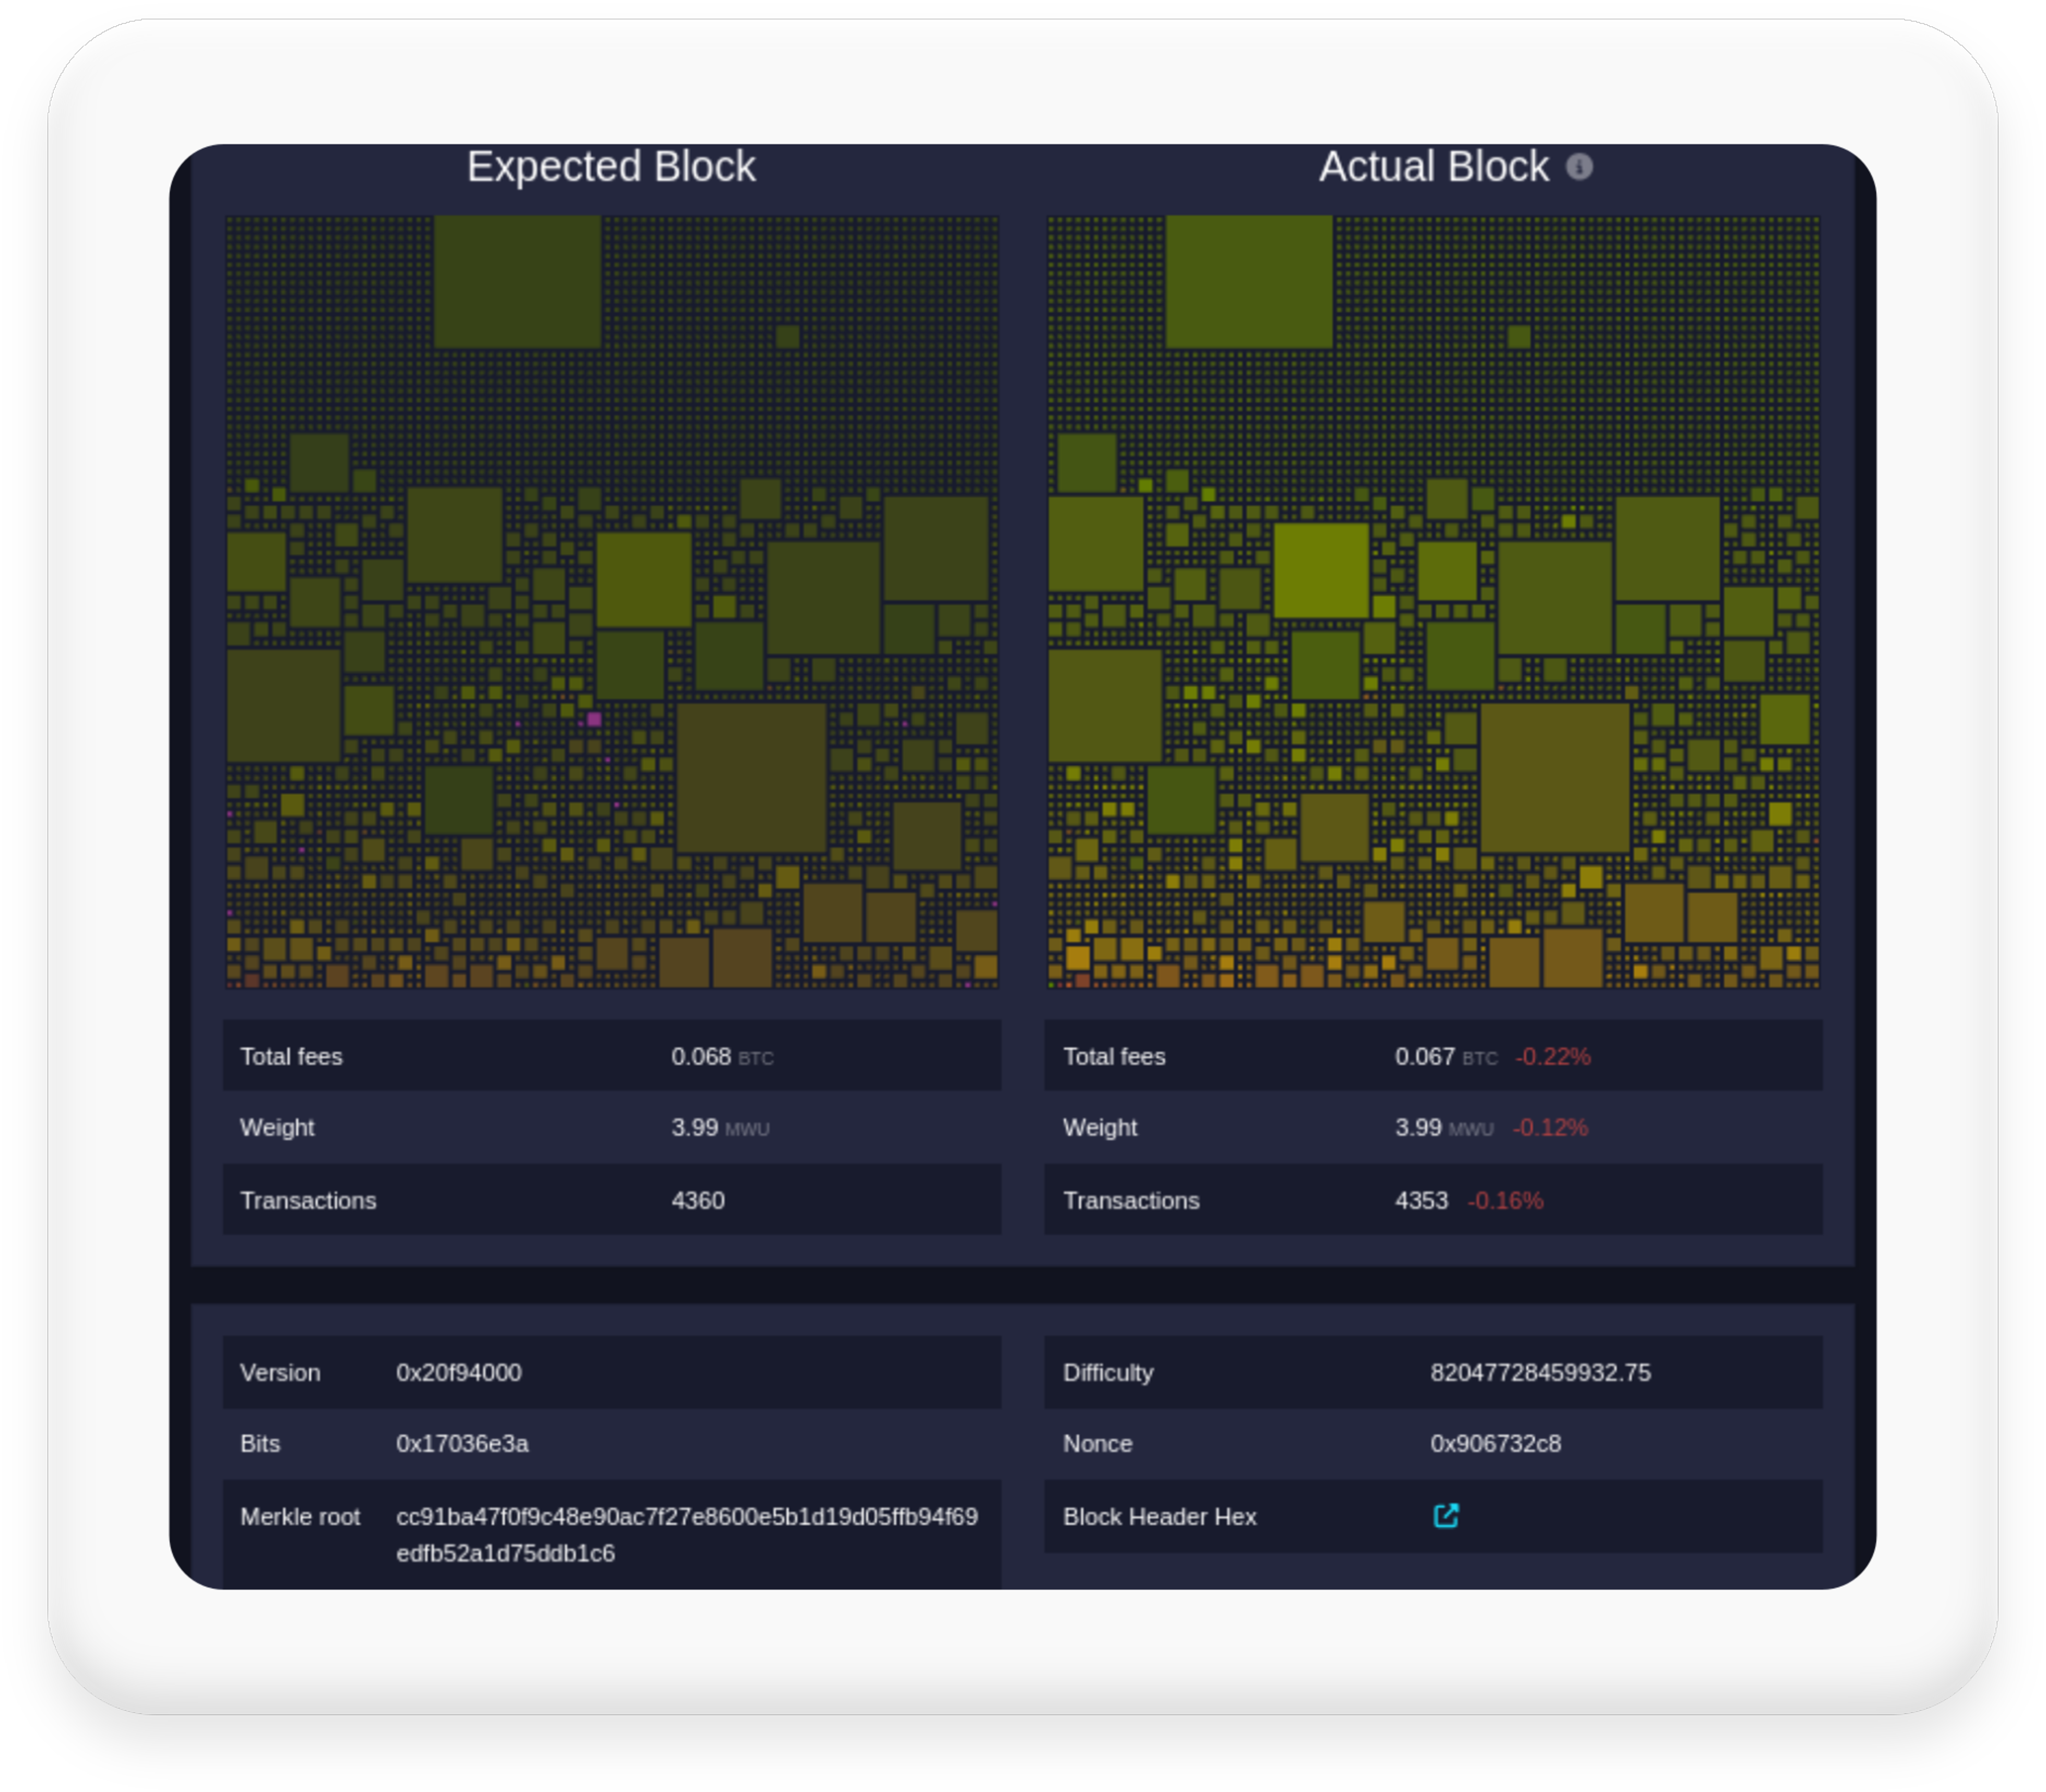
\includegraphics{images/studio/collection/figma-0530-part-01.pdf}}
]{screenshots}
\gdef\studiocataloguename{\detokenize{resource-grid}}
\studiotemplate[
  variant={default},
  palette={light},
  text/1={Resources},
  text/5={Nick Szabo\\Shelling Out: The Origin of Money},
  text/2={Saifedean Ammous\\Bitcoin Standard},
  text/4={Knut Svanholm\\Praxeology},
  text/3={Saifedean Ammous\\Fiat Standard},
  graphic/1={
\includegraphics{images/studio/collection/figma-0563-part-01.pdf}},
  graphic/2={
\includegraphics{images/studio/collection/figma-0563-part-02.pdf}},
  graphic/3={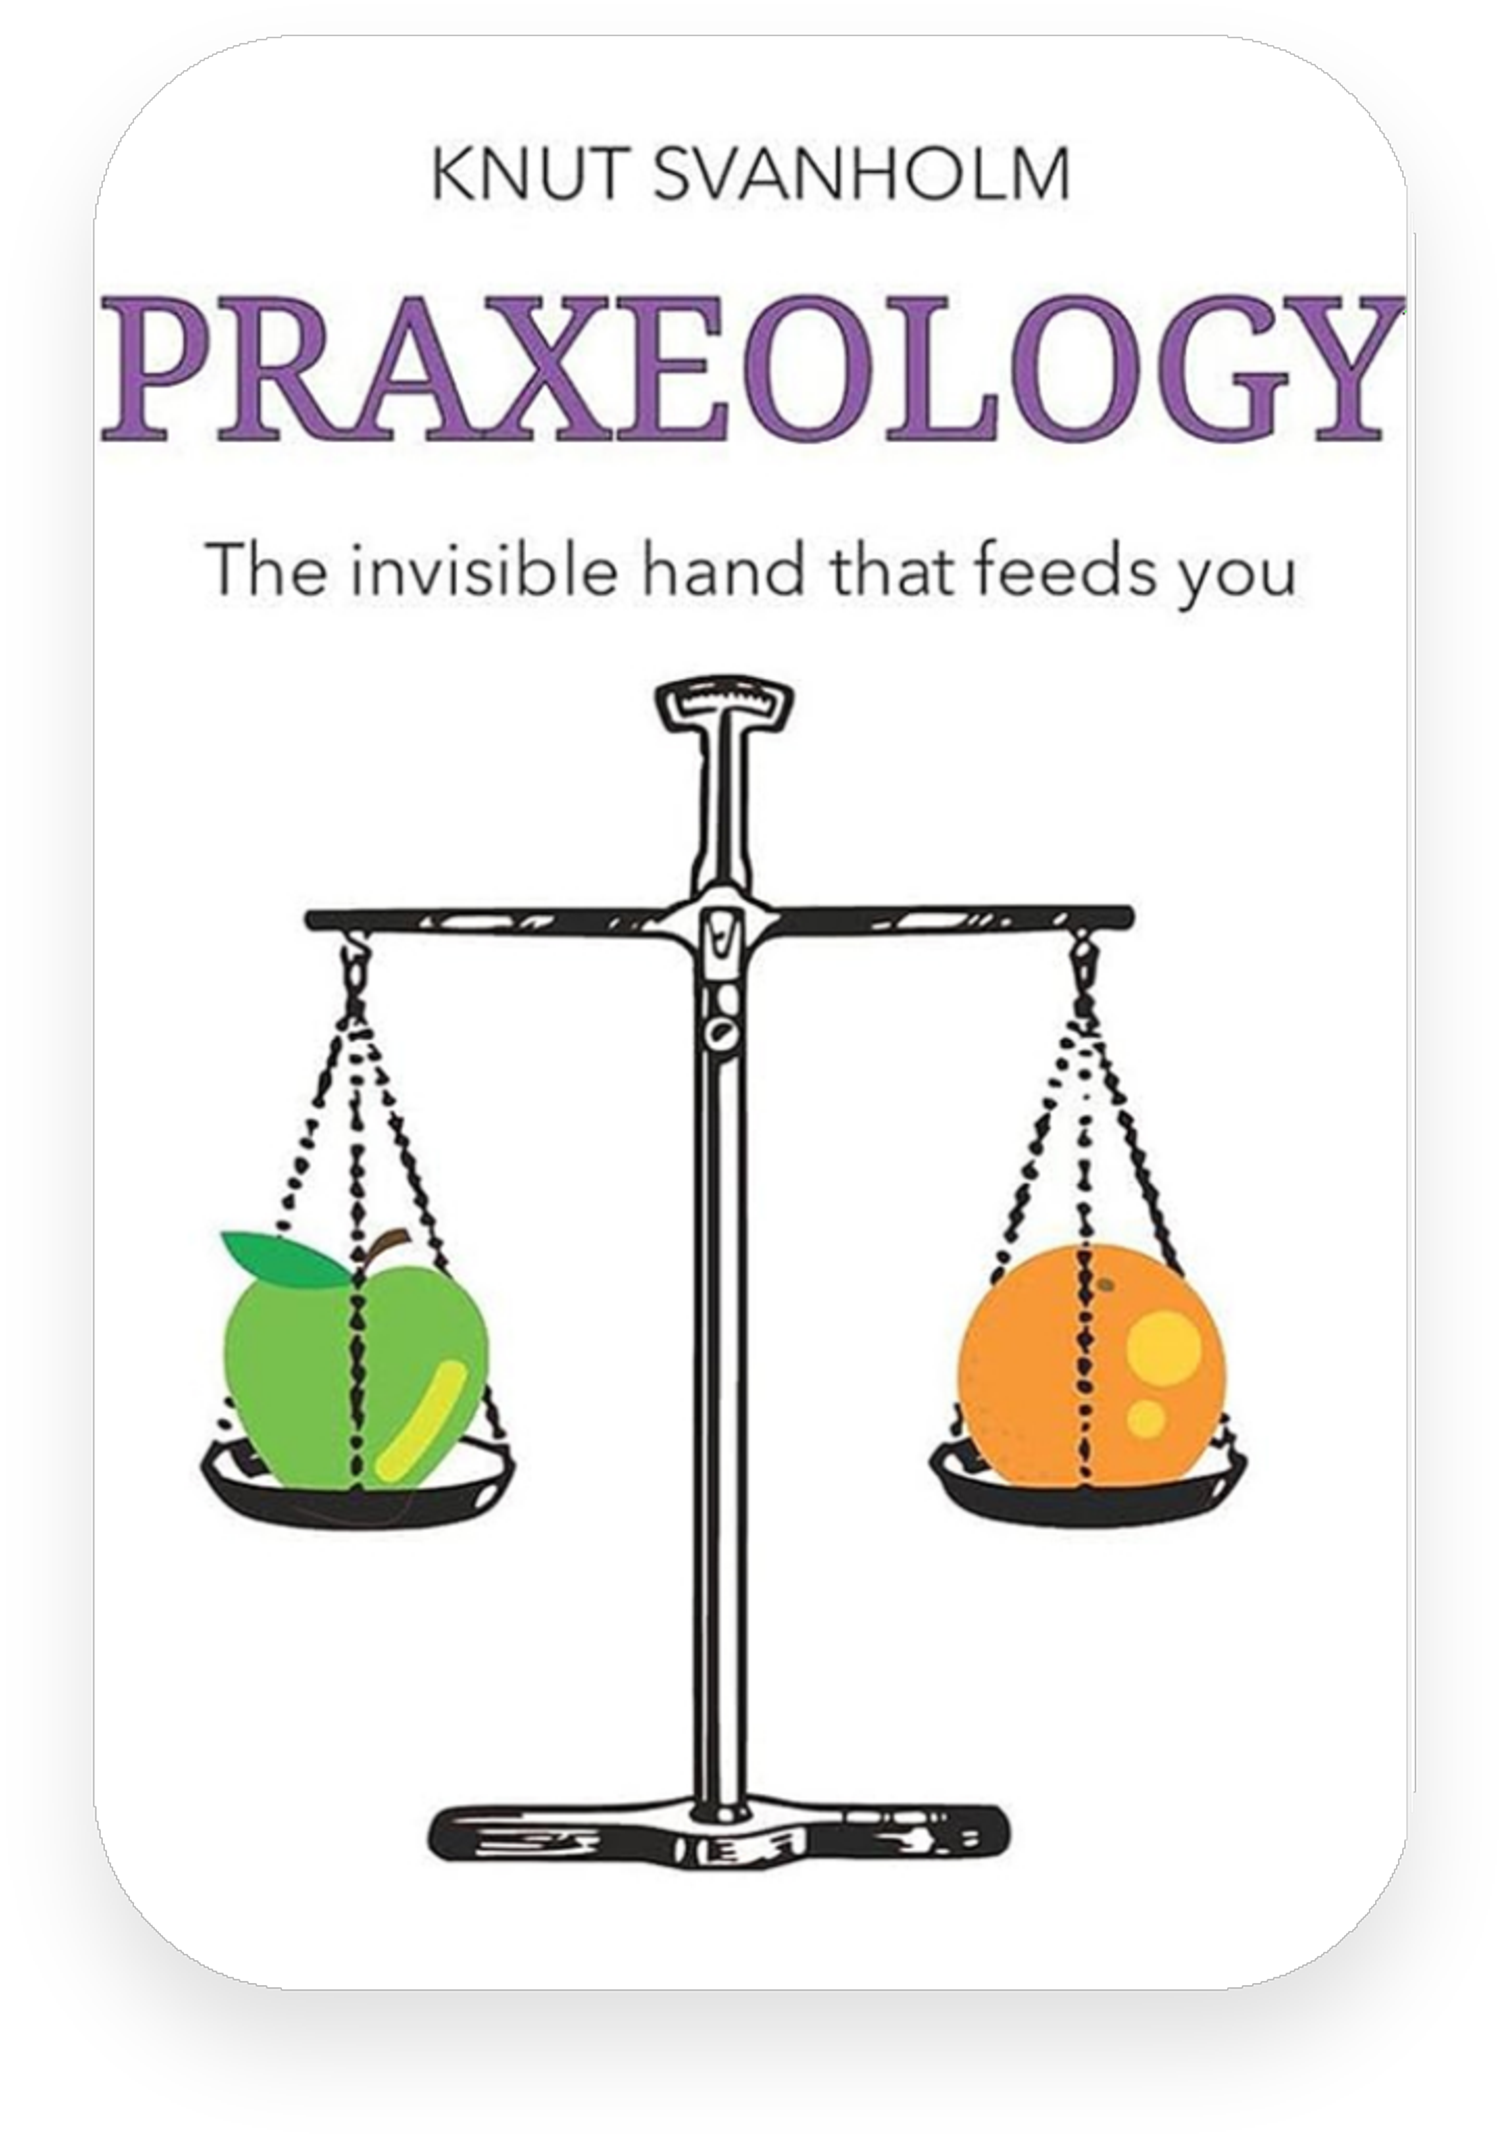
\includegraphics{images/studio/collection/figma-0563-part-03.pdf}},
  graphic/4={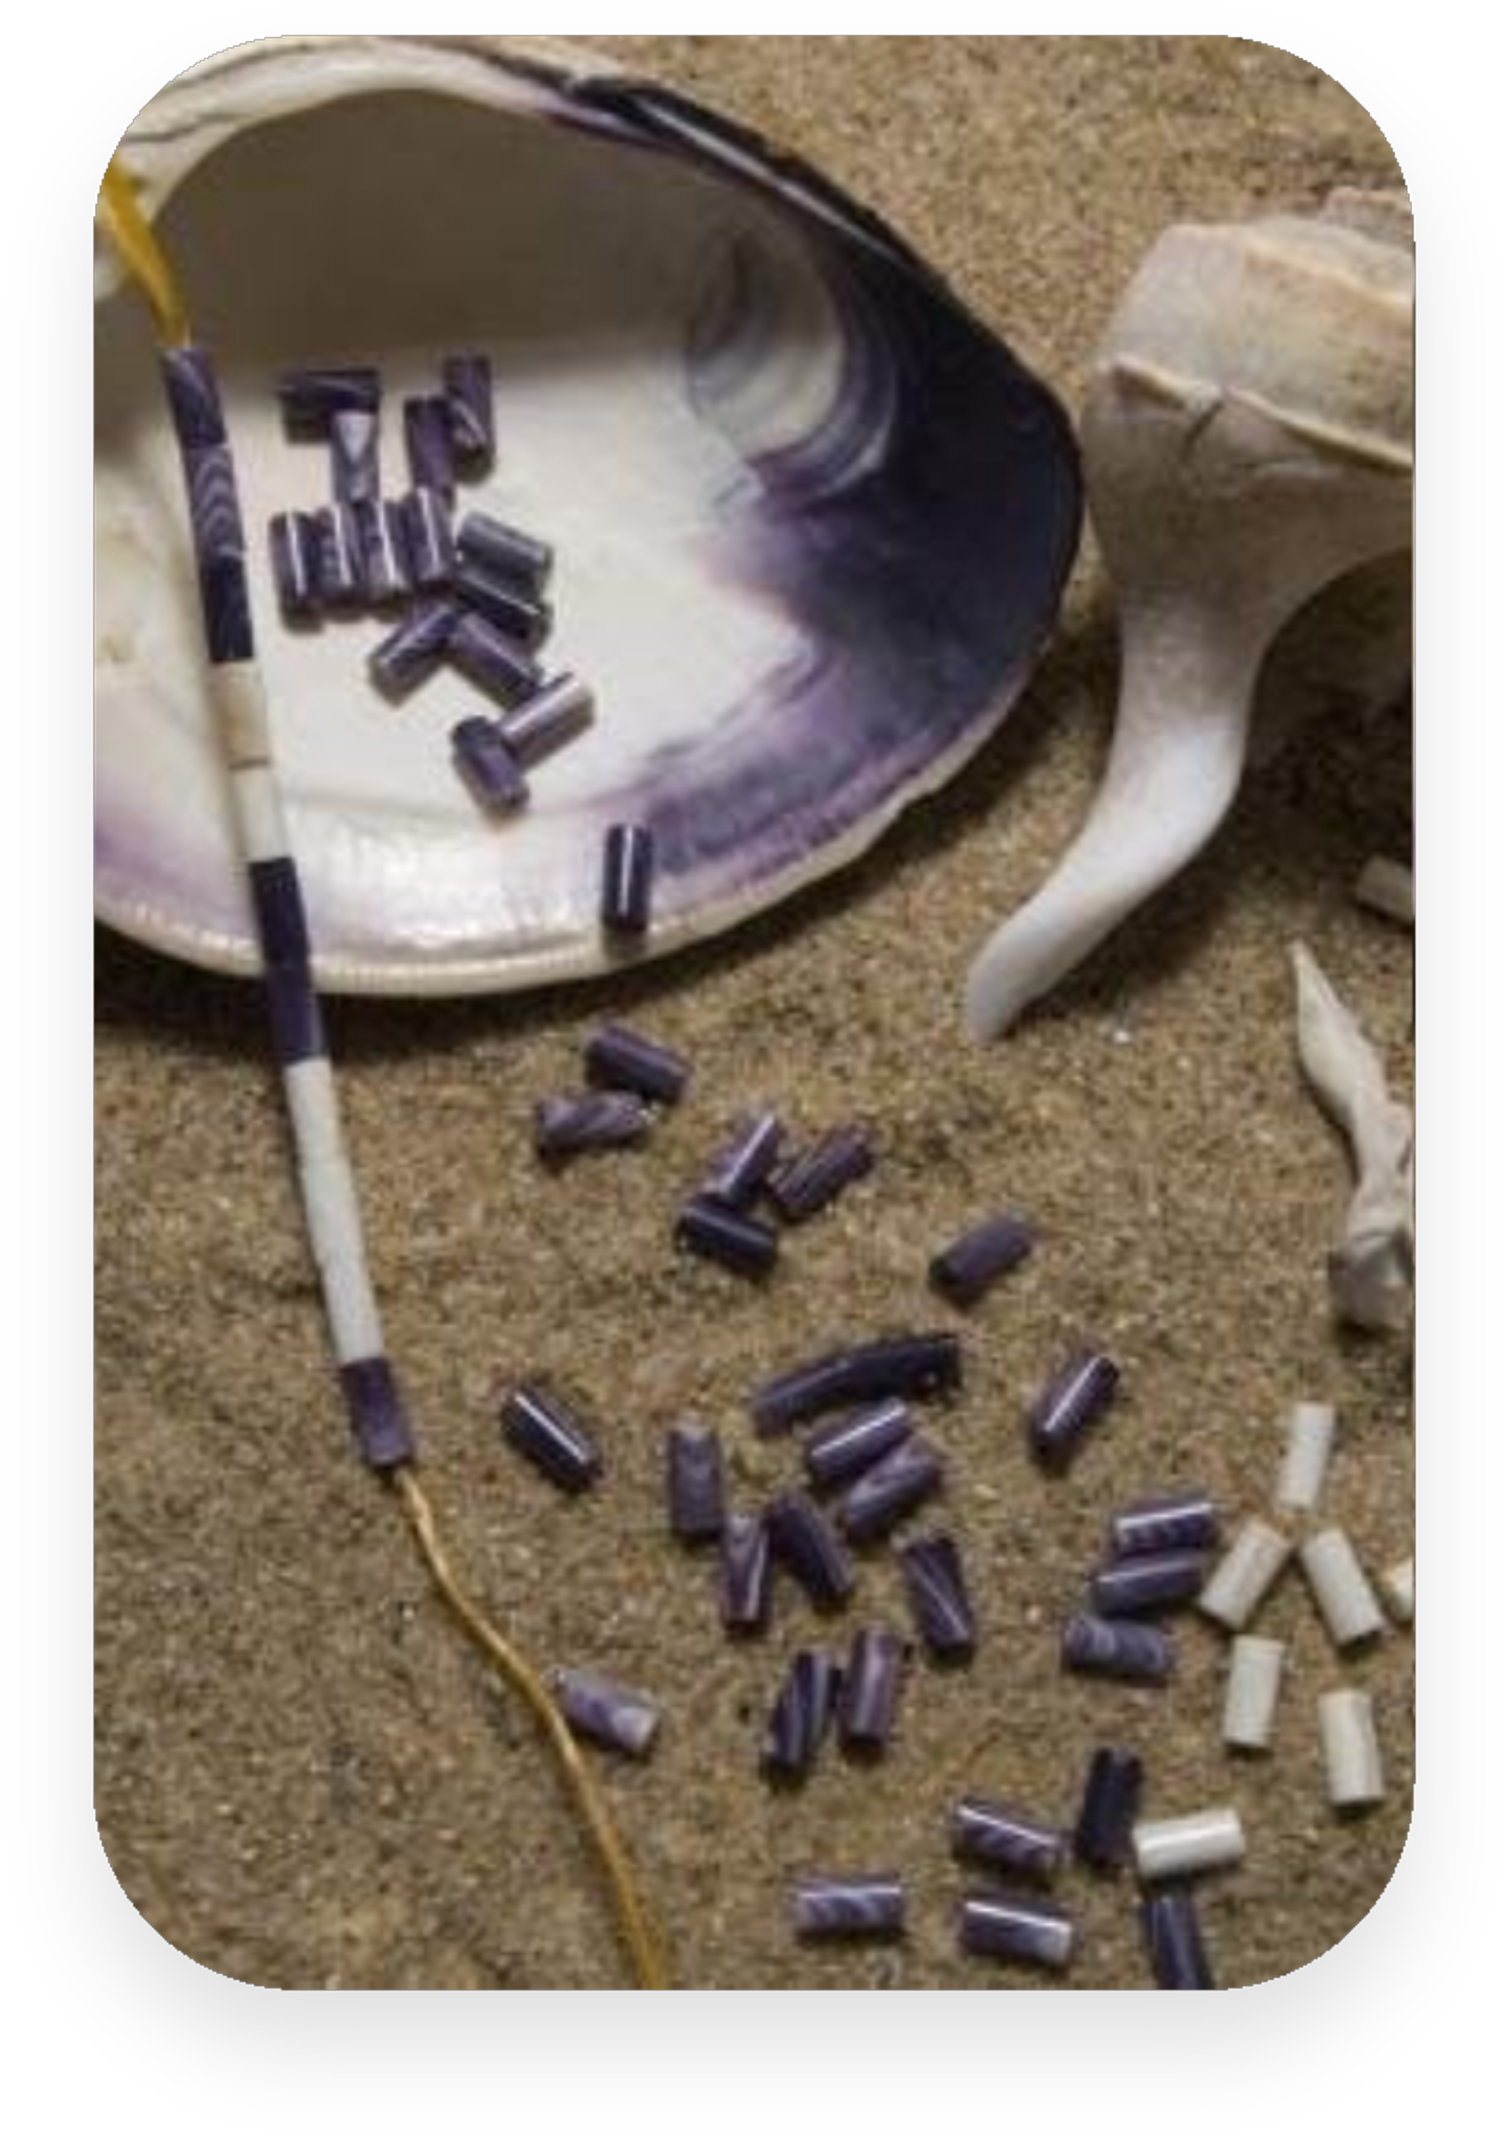
\includegraphics{images/studio/collection/figma-0563-part-04.pdf}}
]{resource-grid}
\gdef\studiocataloguename{\detokenize{photo-collage-banner}}
\studiotemplate[
  variant={banner},
  palette={light}
]{collage}
\gdef\studiocataloguename{\detokenize{photo-collage-grid}}
\studiotemplate[
  variant={grid},
  palette={light},
  text/1={BitPolito in a year}
]{collage}
\gdef\studiocataloguename{\detokenize{photo-triptych}}
\studiotemplate[
  variant={triptych},
  palette={light},
  text/1={Education}
]{image-grid}
\gdef\studiocataloguename{\detokenize{image-pair-title}}
\studiotemplate[
  variant={title-pair},
  palette={light},
  text/1={Central Bank Digital Currency}
]{image-grid}
\gdef\studiocataloguename{\detokenize{nine-logo-grid}}
\studiotemplate[
  variant={default},
  palette={light},
  text/2={BitPofito},
  text/1={Free education},
  graphic/1={
\includegraphics{images/studio/collection/figma-0094-part-01.pdf}},
  graphic/4={
\includegraphics{images/studio/collection/figma-0094-part-02.pdf}},
  graphic/7={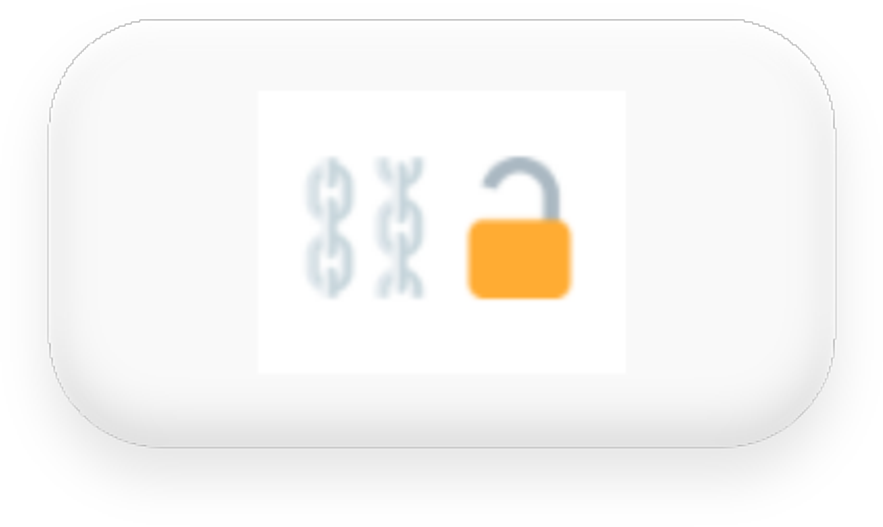
\includegraphics{images/studio/collection/figma-0094-part-03.pdf}},
  graphic/2={
\includegraphics{images/studio/collection/figma-0094-part-04.pdf}},
  graphic/5={
\includegraphics{images/studio/collection/figma-0094-part-05.pdf}},
  graphic/8={
\includegraphics{images/studio/collection/figma-0094-part-06.pdf}},
  graphic/3={
\includegraphics{images/studio/collection/figma-0094-part-07.pdf}},
  graphic/6={
\includegraphics{images/studio/collection/figma-0094-part-08.pdf}},
  graphic/9={
\includegraphics{images/studio/collection/figma-0094-part-09.pdf}}
]{nine-logo-grid}
\gdef\studiocataloguename{\detokenize{screenshot-pair}}
\studiotemplate[
  variant={pair},
  palette={light},
  text/1={LNURLp decode},
  graphic/2={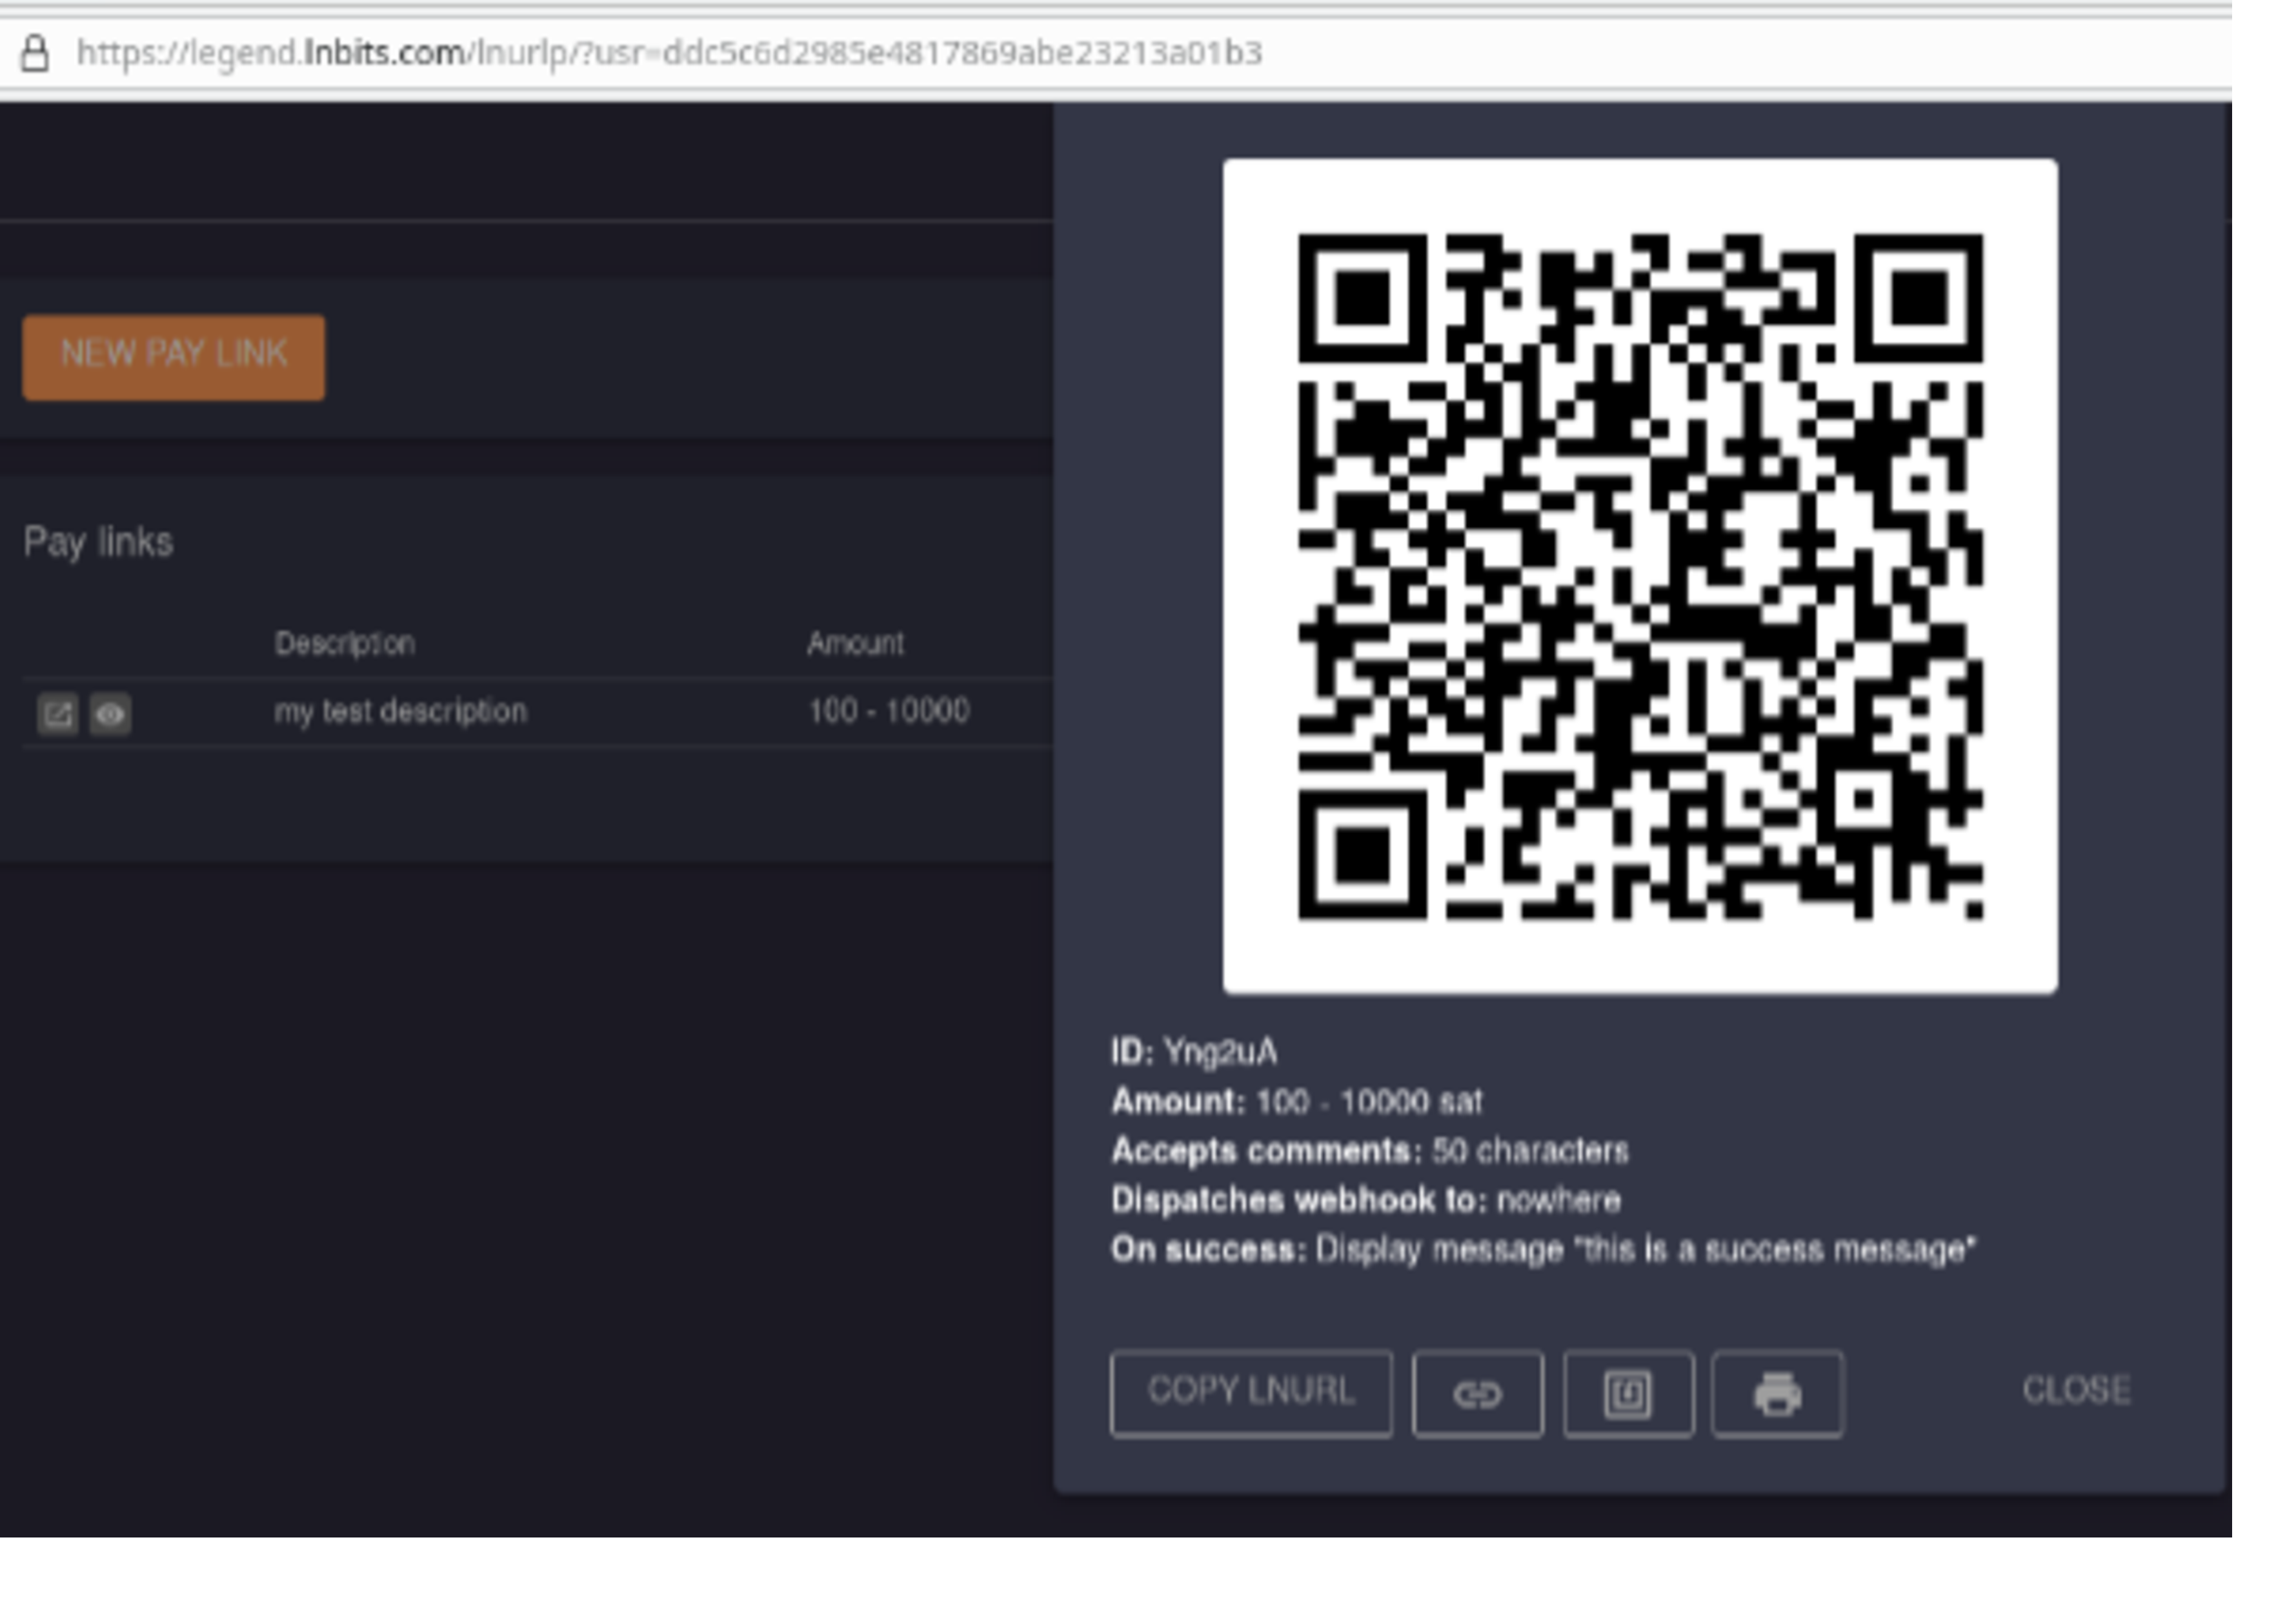
\includegraphics{images/studio/collection/figma-0199-part-01.pdf}},
  graphic/1={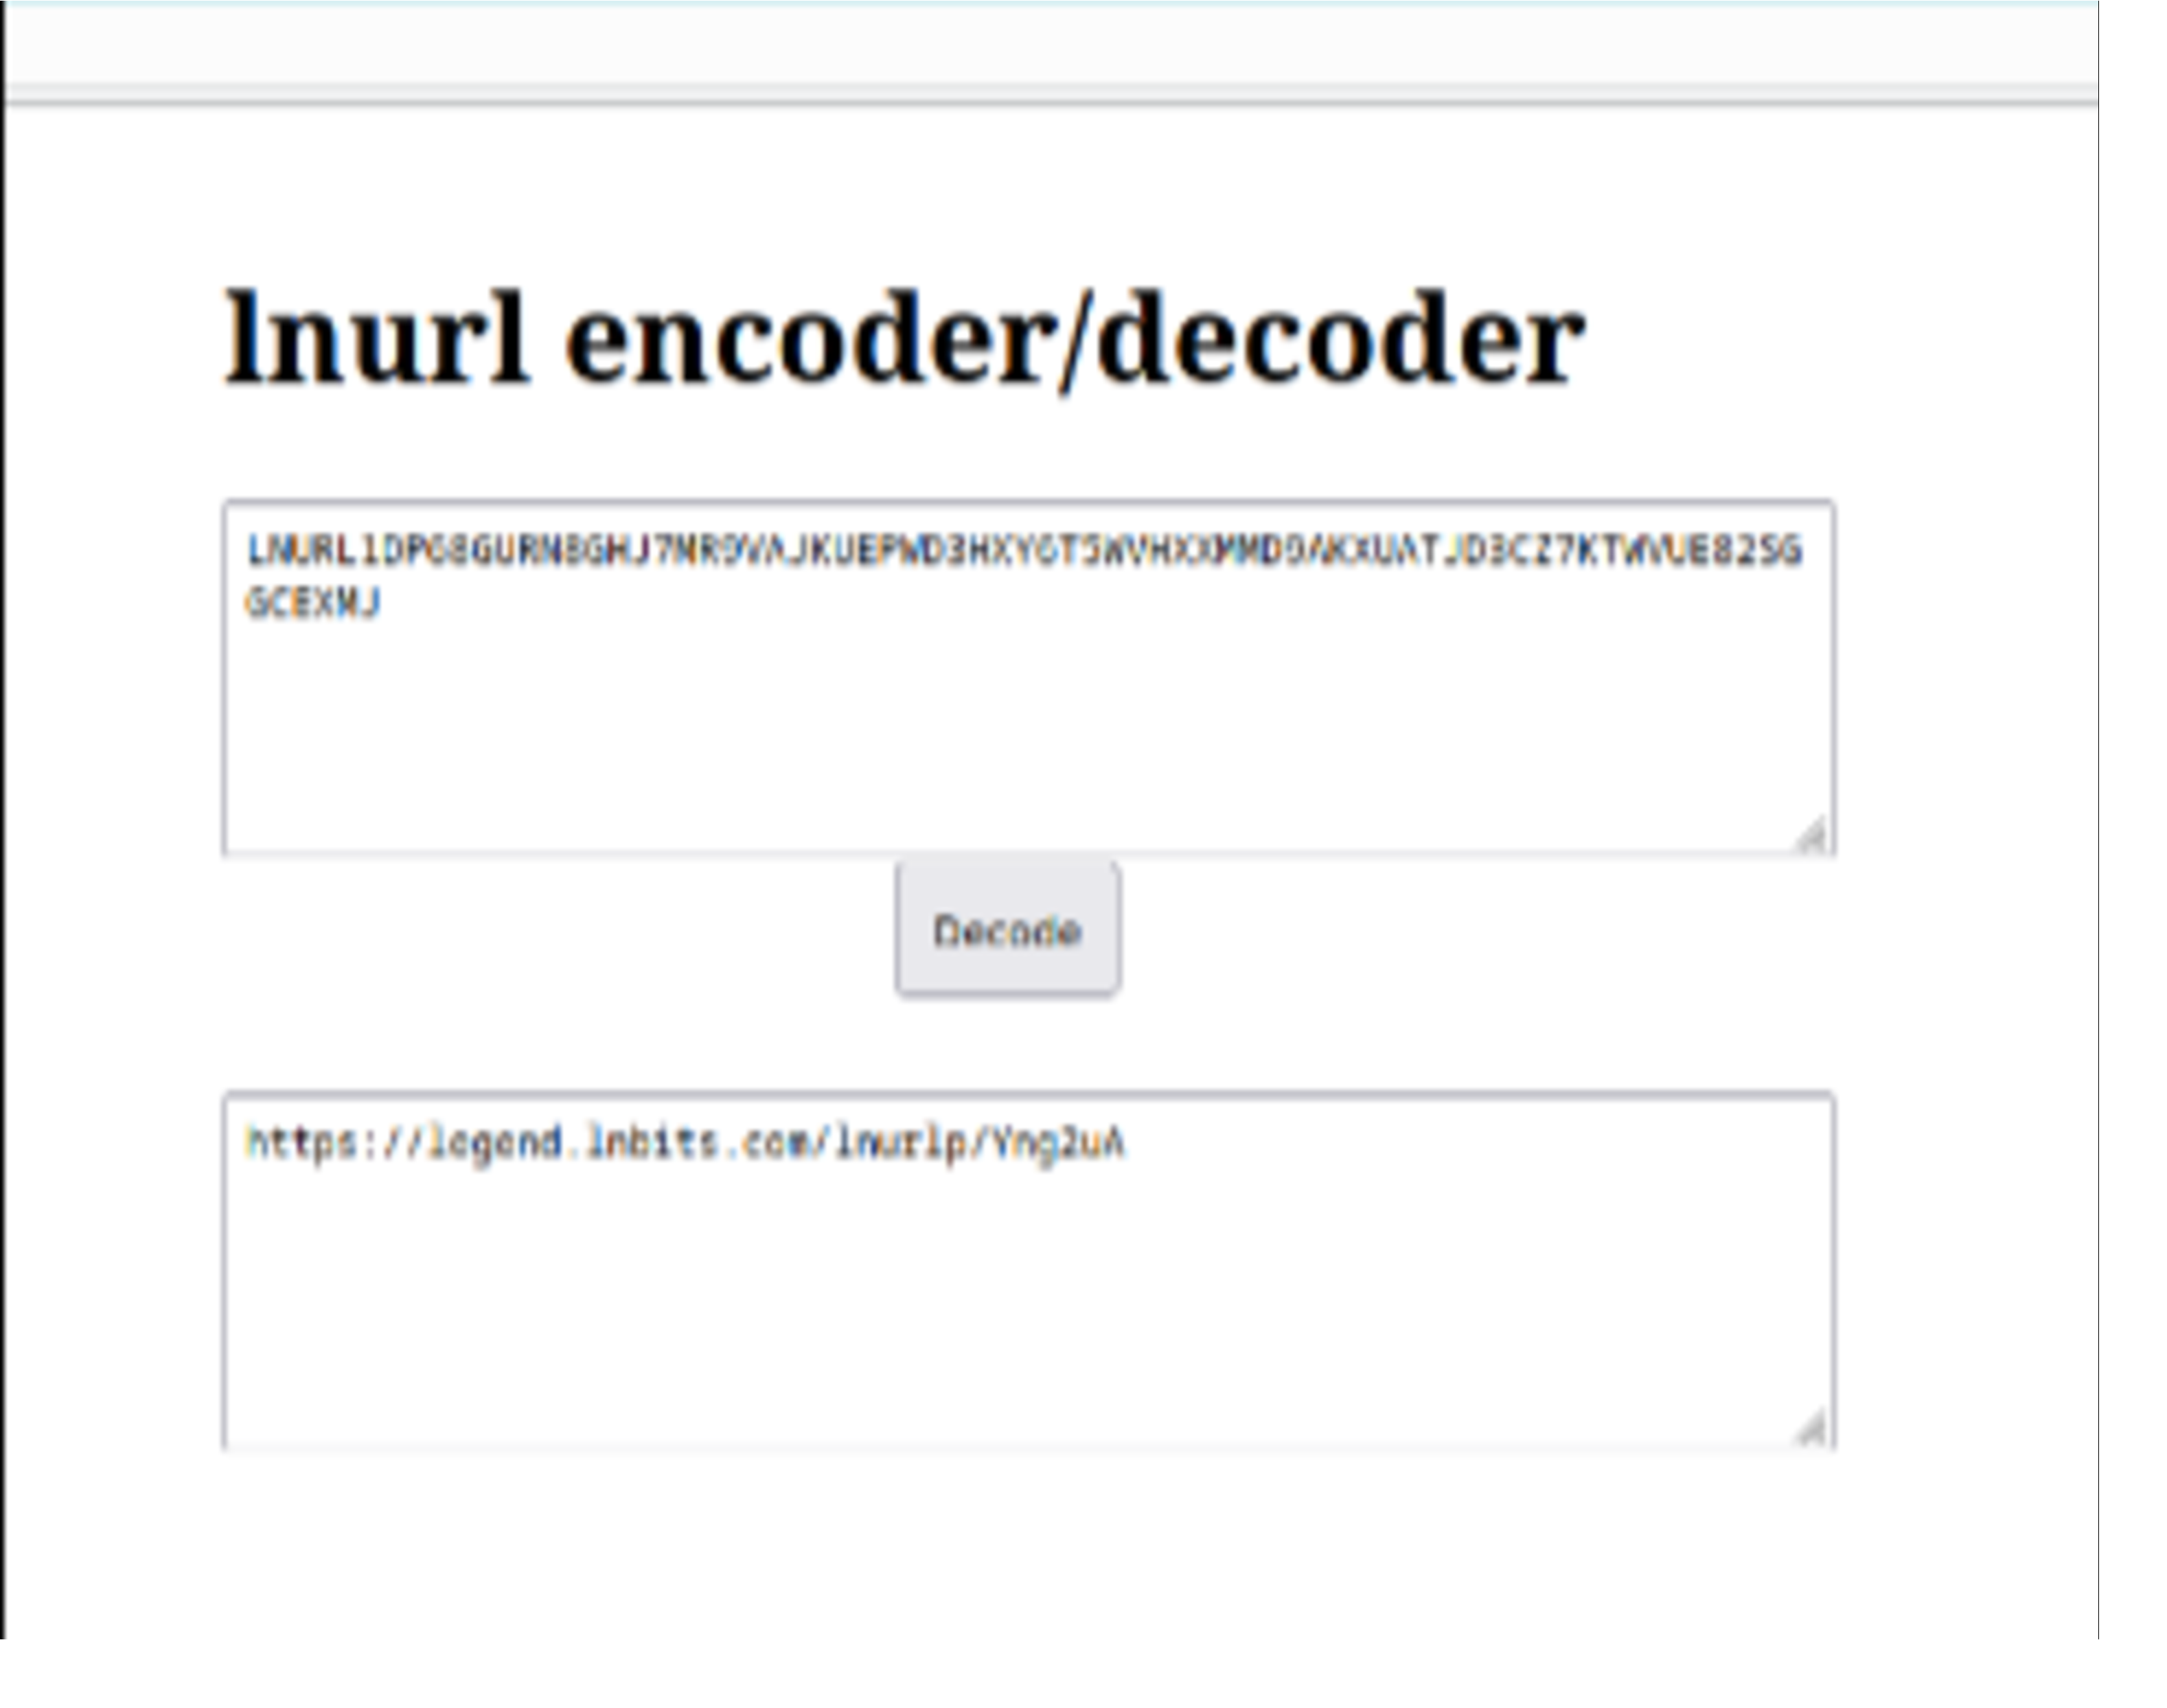
\includegraphics{images/studio/collection/figma-0199-part-02.pdf}}
]{screenshots}
\gdef\studiocataloguename{\detokenize{phone-screenshot}}
\studiotemplate[
  variant={phone},
  palette={light},
  text/1={Amount converted\\and invoice created},
  graphic/1={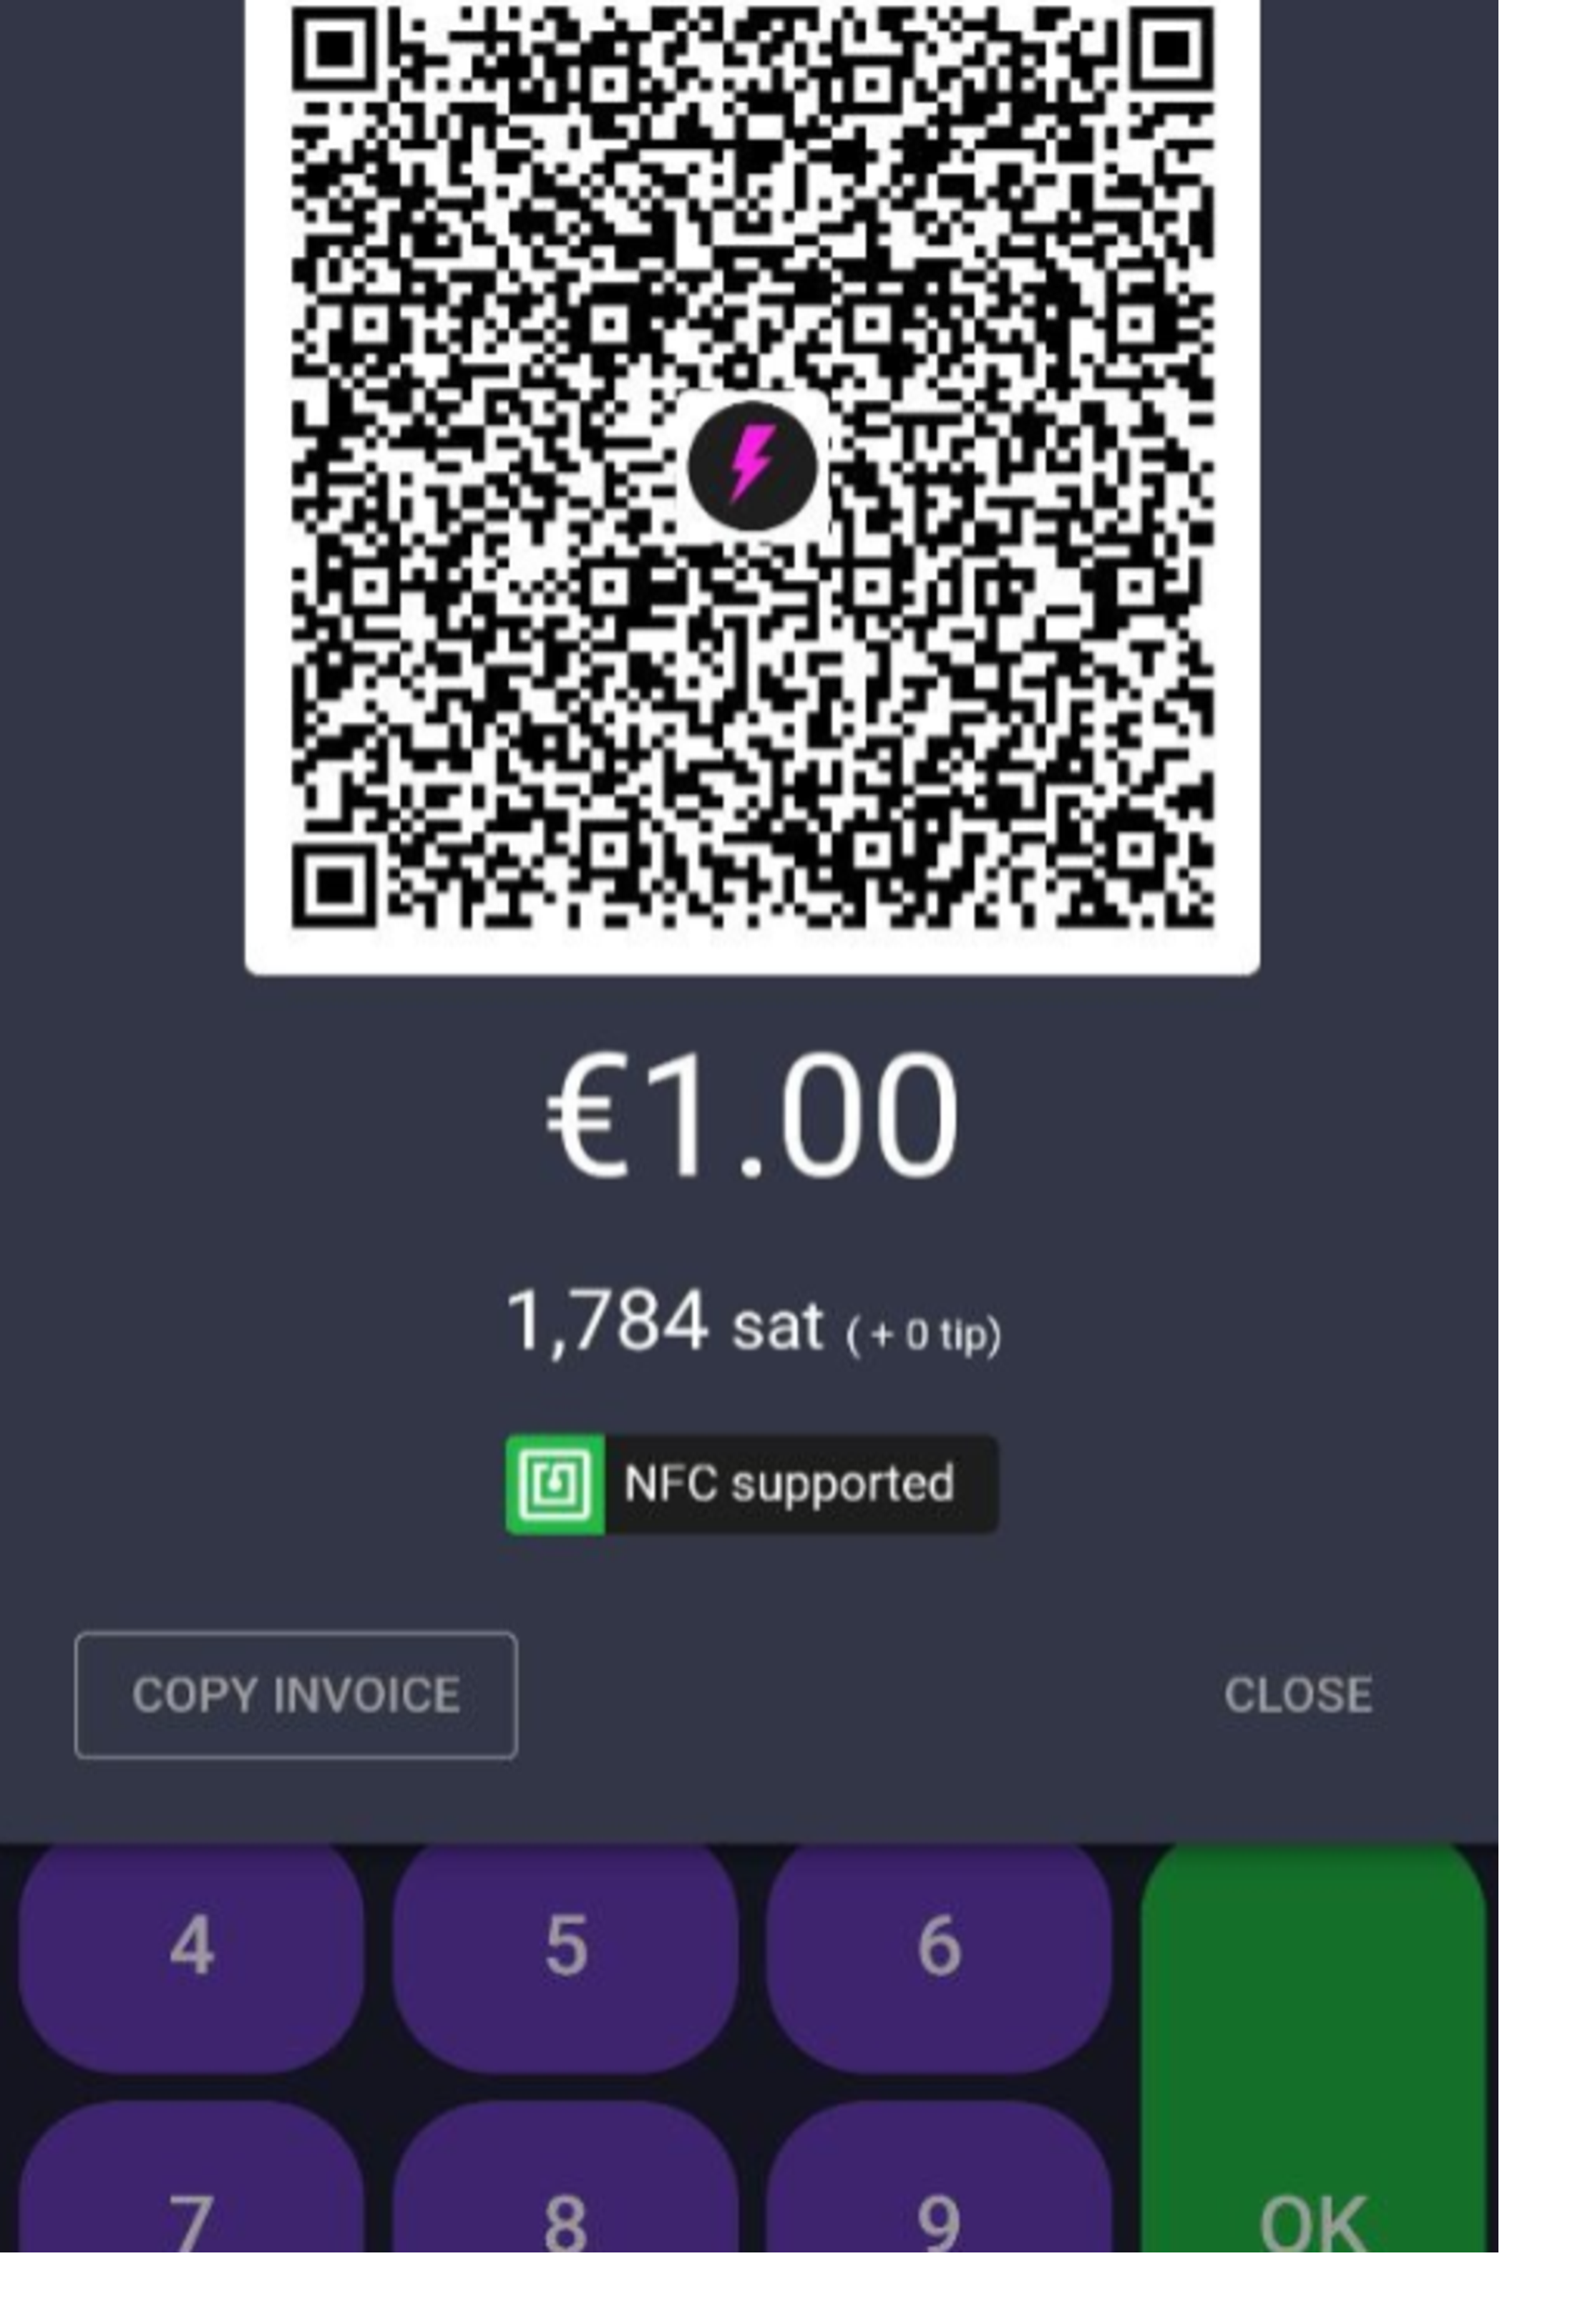
\includegraphics{images/studio/collection/figma-0241-part-01.pdf}}
]{screenshots}
\gdef\studiocataloguename{\detokenize{photo-center-two-icons}}
\studiotemplate[
  variant={default},
  palette={light},
  text/1={``Rules without rulers''}
]{photo-center-two-icons}
\gdef\studiocataloguename{\detokenize{abacus-explanation}}
\studiotemplate[
  variant={default},
  palette={light},
  text/1={The abacus model},
  text/2={Think of a Lightning\\payment channel as\\an abacus: the beads\\represent bitcoin\\inside the channel.}
]{abacus-explanation}
\gdef\studiocataloguename{\detokenize{whitepaper-blue}}
\studiotemplate[
  variant={default},
  palette={blue},
  text/1={Est. 31/10/2008},
  graphic/1={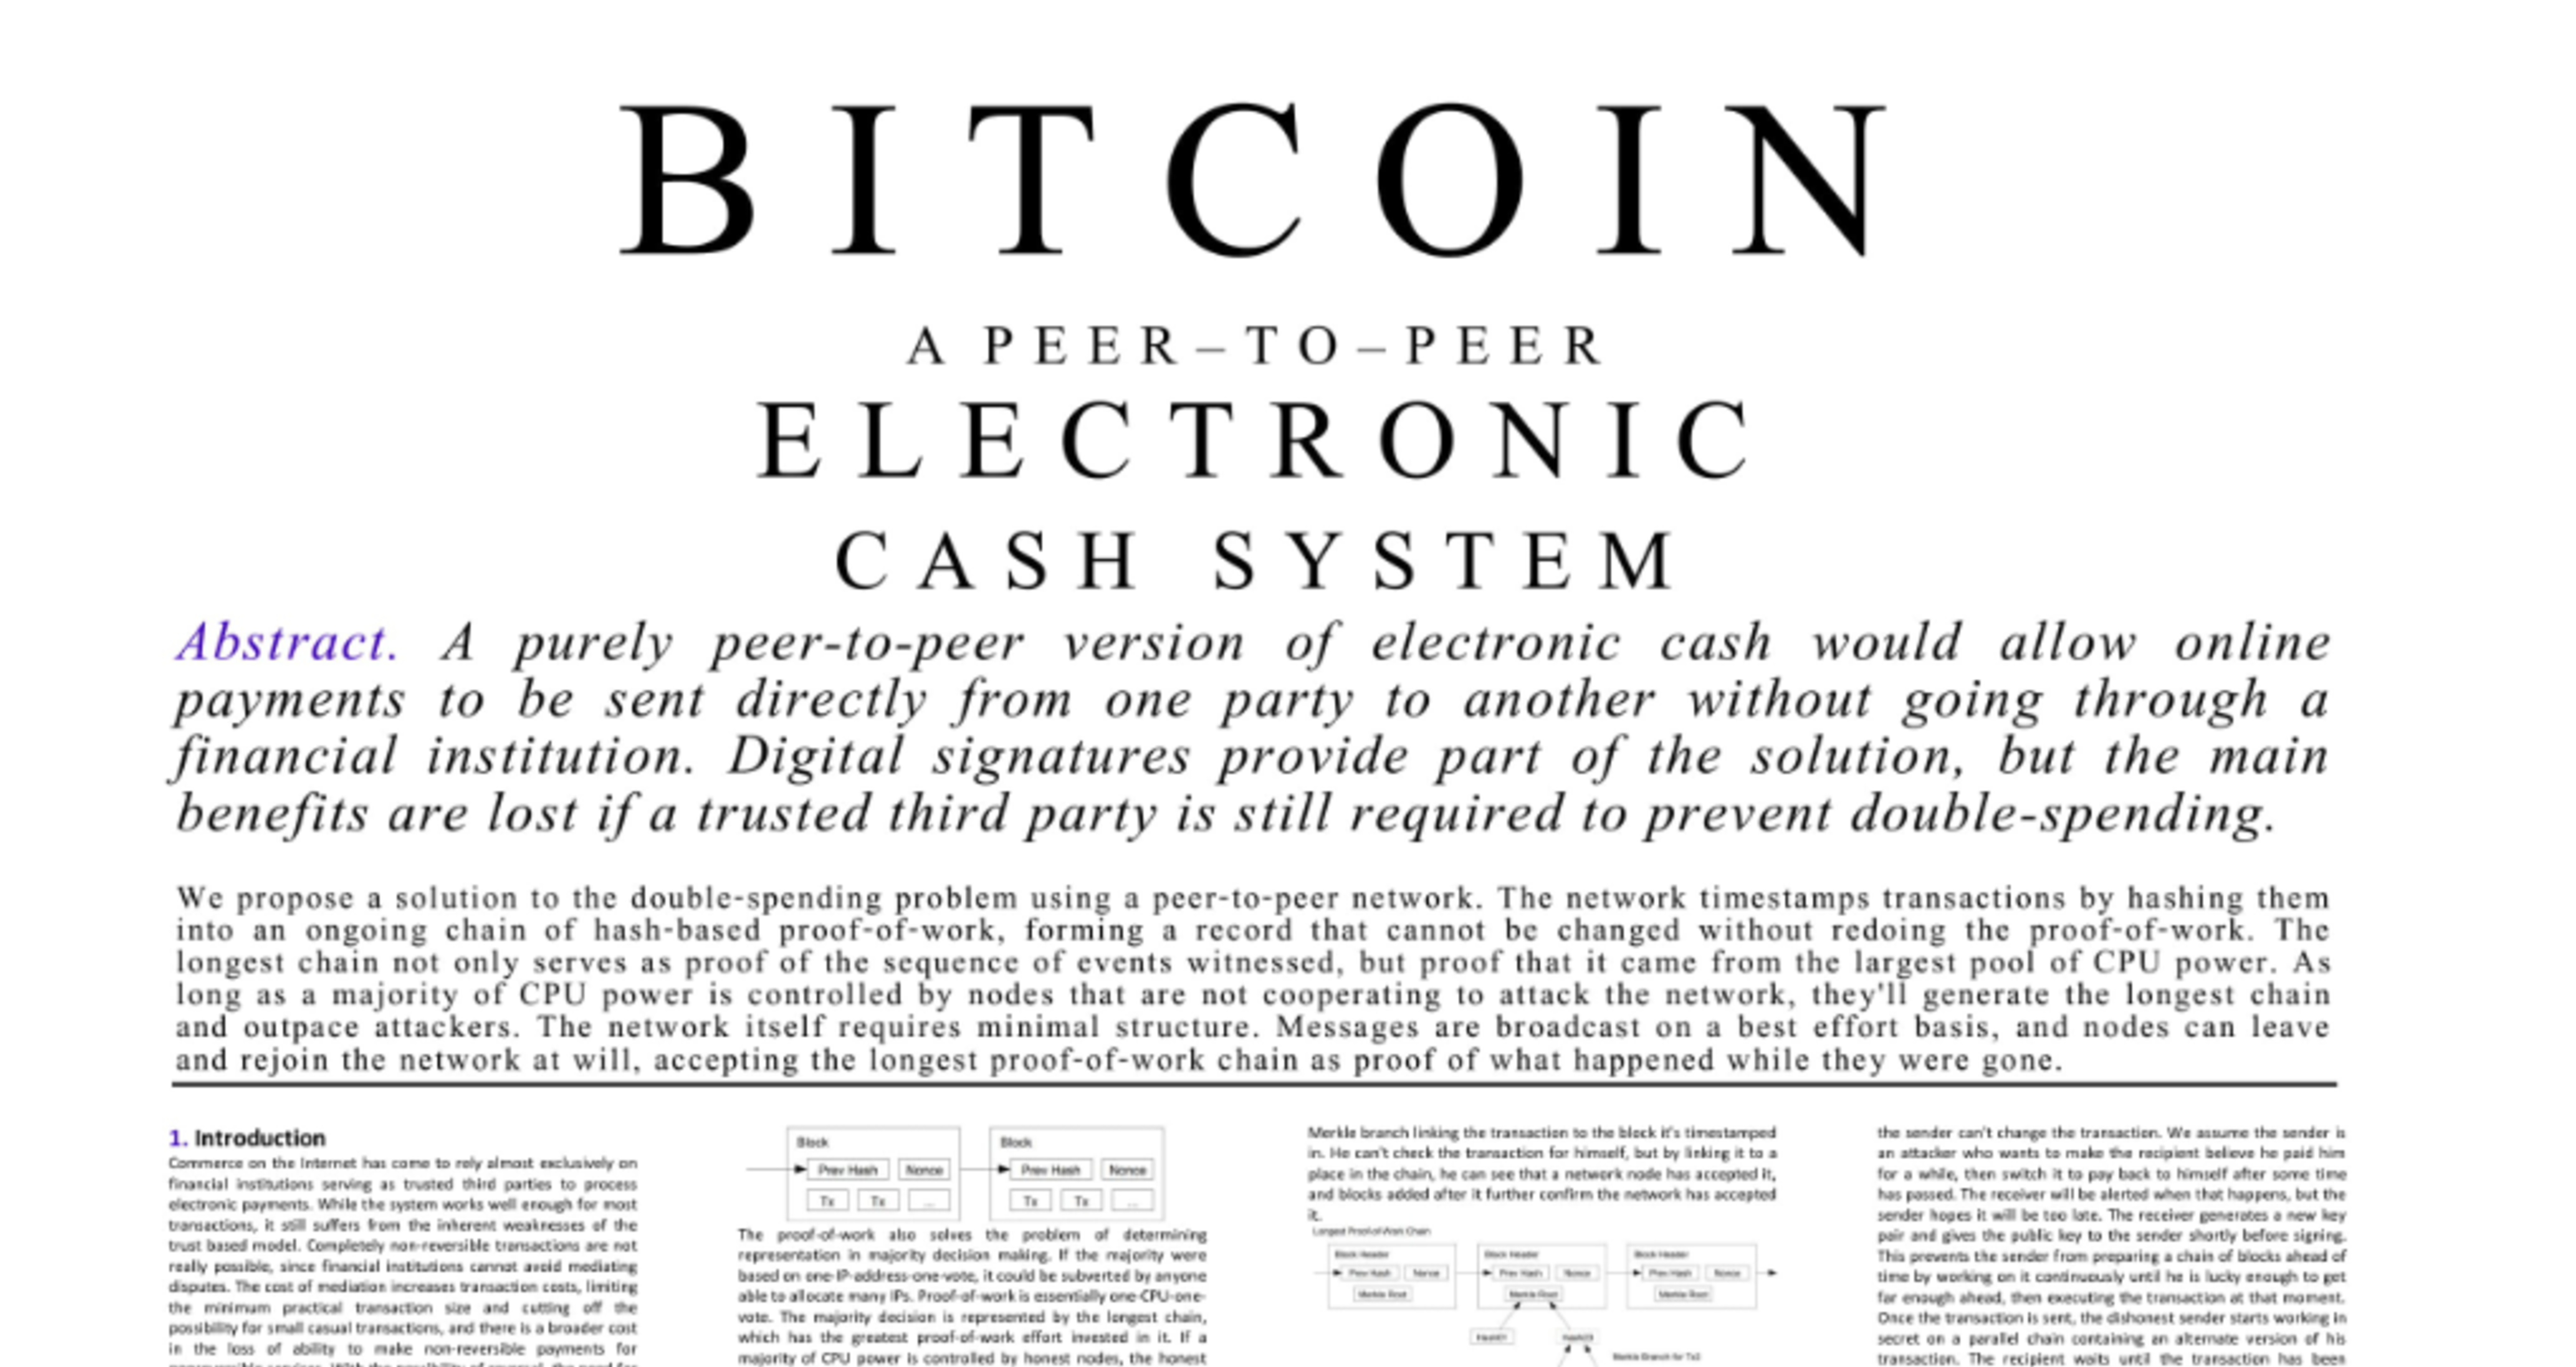
\includegraphics{images/studio/collection/figma-0820-part-01.pdf}}
]{whitepaper-blue}
\gdef\studiocataloguename{\detokenize{partner-media-grid}}
\studiotemplate[
  variant={default},
  palette={light},
  text/10={AZIENDABANGA},
  text/19={e},
  text/24={Information is the asset},
  text/1={Partner, Sponsor \& Media},
  text/2={planb.lugano.ch},
  text/4={@LuganoPlanB},
  text/3={bitbox.swiss},
  text/5={@BitBoxSwiss},
  text/6={zebedee.io},
  text/8={@zbdapp},
  text/7={stratumprotocol.org},
  text/9={@StratumV2},
  text/11={fulgur.ventures},
  text/13={@fulgurventures},
  text/12={relai.app},
  text/14={@relai\_app},
  text/15={braiins.com},
  text/17={@BraiinsMining},
  text/16={vex\.it},
  text/18={@vexl},
  text/20={blockstream.com},
  text/22={@Blockstream},
  text/21={planb.network},
  text/23={@planb\_network},
  graphic/1={
\includegraphics{images/studio/collection/figma-0930-part-01.pdf}},
  graphic/28={
\includegraphics{images/studio/collection/figma-0930-part-02.pdf}},
  graphic/20={
\includegraphics{images/studio/collection/figma-0930-part-03.pdf}},
  graphic/21={
\includegraphics{images/studio/collection/figma-0930-part-04.pdf}},
  graphic/33={
\includegraphics{images/studio/collection/figma-0930-part-05.pdf}},
  graphic/2={
\includegraphics{images/studio/collection/figma-0930-part-06.pdf}},
  graphic/3={
\includegraphics{images/studio/collection/figma-0930-part-07.pdf}},
  graphic/6={
\includegraphics{images/studio/collection/figma-0930-part-08.pdf}},
  graphic/4={
\includegraphics{images/studio/collection/figma-0930-part-09.pdf}},
  graphic/5={
\includegraphics{images/studio/collection/figma-0930-part-10.pdf}},
  graphic/7={
\includegraphics{images/studio/collection/figma-0930-part-11.pdf}},
  graphic/8={
\includegraphics{images/studio/collection/figma-0930-part-12.pdf}},
  graphic/9={
\includegraphics{images/studio/collection/figma-0930-part-13.pdf}},
  graphic/12={
\includegraphics{images/studio/collection/figma-0930-part-14.pdf}},
  graphic/10={
\includegraphics{images/studio/collection/figma-0930-part-15.pdf}},
  graphic/11={
\includegraphics{images/studio/collection/figma-0930-part-16.pdf}},
  graphic/13={
\includegraphics{images/studio/collection/figma-0930-part-17.pdf}},
  graphic/14={
\includegraphics{images/studio/collection/figma-0930-part-18.pdf}},
  graphic/15={
\includegraphics{images/studio/collection/figma-0930-part-19.pdf}},
  graphic/18={
\includegraphics{images/studio/collection/figma-0930-part-20.pdf}},
  graphic/16={
\includegraphics{images/studio/collection/figma-0930-part-21.pdf}},
  graphic/17={
\includegraphics{images/studio/collection/figma-0930-part-22.pdf}},
  graphic/19={
\includegraphics{images/studio/collection/figma-0930-part-23.pdf}},
  graphic/22={
\includegraphics{images/studio/collection/figma-0930-part-24.pdf}},
  graphic/24={
\includegraphics{images/studio/collection/figma-0930-part-25.pdf}},
  graphic/26={
\includegraphics{images/studio/collection/figma-0930-part-26.pdf}},
  graphic/23={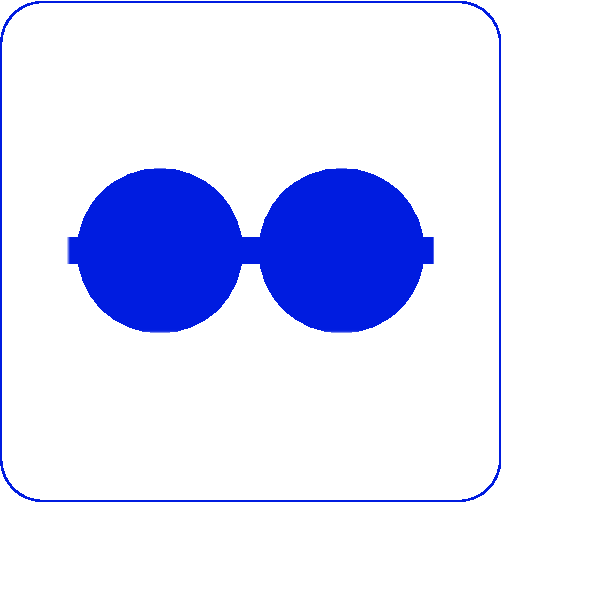
\includegraphics{images/studio/collection/figma-0930-part-27.pdf}},
  graphic/25={
\includegraphics{images/studio/collection/figma-0930-part-28.pdf}},
  graphic/27={
\includegraphics{images/studio/collection/figma-0930-part-29.pdf}},
  graphic/29={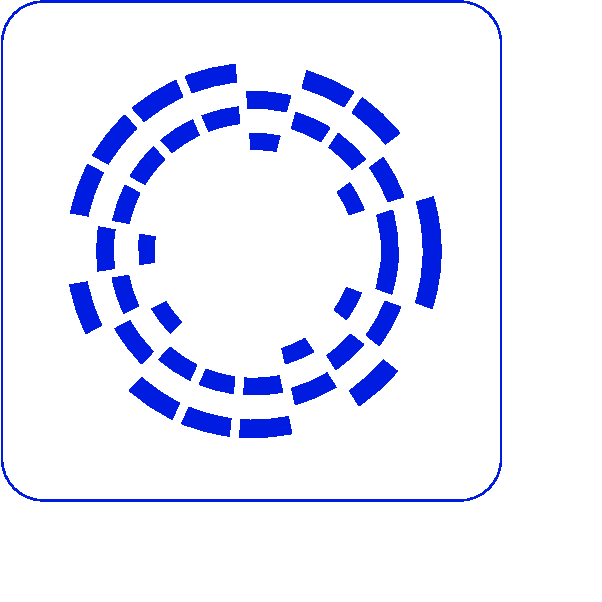
\includegraphics{images/studio/collection/figma-0930-part-30.pdf}},
  graphic/30={
\includegraphics{images/studio/collection/figma-0930-part-31.pdf}},
  graphic/34={
\includegraphics{images/studio/collection/figma-0930-part-32.pdf}},
  graphic/31={
\includegraphics{images/studio/collection/figma-0930-part-33.pdf}},
  graphic/32={
\includegraphics{images/studio/collection/figma-0930-part-34.pdf}},
  graphic/35={
\includegraphics{images/studio/collection/figma-0930-part-35.pdf}}
]{partner-media-grid}
\gdef\studiocataloguename{\detokenize{mission-badges}}
\studiotemplate[
  variant={default},
  palette={light},
  text/4={Lugano\\October 25-26},
  text/2={Cuneo},
  text/5={March 22},
  text/3={Brescia\\May 10},
  text/6={9 conference as speaker in 2025},
  text/1={Missions}
]{mission-badges}
\gdef\studiocataloguename{\detokenize{image-logo-pair}}
\studiotemplate[
  variant={default},
  palette={light},
  text/1={Satoshi Spritz},
  text/2={Einundzwanzig fork},
  graphic/1={
\includegraphics{images/studio/collection/figma-0538-part-01.pdf}}
]{image-logo-pair}
\section{Data}
\gdef\studiocataloguename{\detokenize{hero-number}}
\studiotemplate[
  variant={default},
  palette={light},
  text/1={21.000.000},
  text/2={A finite number of monetary units (hard cap)}
]{hero-number}
\gdef\studiocataloguename{\detokenize{three-statistics}}
\studiotemplate[
  variant={four-counters},
  palette={light},
  text/1={Mining},
  text/6={BTC already mined},
  text/3={94,3\%},
  text/11={BTC mined per day},
  text/9={450},
  text/5={BTC already mined},
  text/2={19,8 M},
  text/10={BTC remaining},
  text/8={1,2M},
  text/4={Issue new bitcoin},
  text/7={Confirm new transactions},
  text/12={Secure the network}
]{metrics}
\gdef\studiocataloguename{\detokenize{line-chart}}
\studiotemplate[
  variant={line},
  palette={light},
  text/1={Peak hashrate},
  text/2={1.039 ZH/s*},
  text/3={35,7 \%},
  text/4={*815 ha of 1,000 W bulbs}
]{charts}
\gdef\studiocataloguename{\detokenize{diagonal-number}}
\studiotemplate[
  variant={default},
  palette={blue},
  text/1={Fixed supply}
]{diagonal-number}
\gdef\studiocataloguename{\detokenize{unit-conversion}}
\studiotemplate[
  variant={default},
  palette={light},
  text/4={100,000,000},
  text/2={satoshi},
  text/3={bitcoin},
  text/5={1.00000000},
  text/6={00000000.1},
  text/1={Units of measurement}
]{unit-conversion}
\gdef\studiocataloguename{\detokenize{bar-comparison}}
\studiotemplate[
  variant={bars},
  palette={light},
  text/24={Ukraine},
  text/25={14.4},
  text/15={Bangladesh},
  text/23={15.5},
  text/18={Vietnam},
  text/19={15.9},
  text/13={Pakistan},
  text/17={21.0},
  text/22={vs. 2023},
  text/21={Nigeria},
  text/14={24.3},
  text/11={28.9},
  text/10={Egypt},
  text/9={33.8},
  text/8={Philippines},
  text/7={35.7},
  text/6={Mexico},
  text/5={67.4},
  text/2={India},
  text/3={78.6},
  text/4={China},
  text/26={Source: World Bank},
  text/1={Top remittance recipients in 2024},
  text/16={Billion transferred},
  text/12={\$905},
  text/20={+4.5\%}
]{charts}
\gdef\studiocataloguename{\detokenize{scatter-comparison}}
\studiotemplate[
  variant={scatter},
  palette={light},
  text/7={50},
  text/8={100},
  text/9={Simplicity},
  text/1={Methods compared},
  text/2={P2P},
  text/6={Banks and TradFi},
  text/5={Exchange},
  text/4={ATM},
  text/3={App Bitcoin}
]{charts}
\gdef\studiocataloguename{\detokenize{adoption-curve}}
\studiotemplate[
  variant={stages},
  palette={light},
  text/2={Innovators},
  text/6={Laggards},
  text/3={Early\\adopters},
  text/4={Early\\majority},
  text/5={Late\\majority},
  text/1={Chasm},
  text/7={3\%},
  text/8={13\%},
  text/9={34\%},
  text/10={34\%},
  text/11={16\%}
]{charts}
\gdef\studiocataloguename{\detokenize{metric-dashboard}}
\studiotemplate[
  variant={four-panels},
  palette={light},
  text/6={Key Metrics},
  text/1={50},
  text/3={Participants},
  text/2={140},
  text/4={Alumni},
  text/5={\textasciitilde6000},
  text/7={Social media followers},
  text/8={30+},
  text/9={Events organized}
]{metrics}
\gdef\studiocataloguename{\detokenize{ranked-podium}}
\studiotemplate[
  variant={default},
  palette={light},
  text/1={Game theory},
  text/2={Winner takes all effect},
  text/3={Lindy effect},
  text/6={LOW},
  text/7={NEW},
  text/8={OLD},
  text/5={HIGH},
  text/4={Life expectancy},
  text/9={Time being around}
]{ranked-podium}
\gdef\studiocataloguename{\detokenize{two-charts}}
\studiotemplate[
  variant={two},
  palette={light},
  text/6={1920},
  text/7={1930},
  text/8={1940},
  text/9={1950},
  text/10={1960},
  text/11={1970},
  text/12={1980},
  text/13={1990},
  text/14={2000},
  text/15={2010},
  text/16={2020},
  text/1={Monetary expansion},
  text/28={Source: US Fed},
  text/3={Billions of dollars},
  text/5={Ke)\\An},
  text/17={1920},
  text/18={1930},
  text/19={1940},
  text/20={1950},
  text/21={1960},
  text/22={1970},
  text/23={1980},
  text/24={1990},
  text/25={2000},
  text/26={2010},
  text/27={2020},
  text/2={Purchasing power},
  text/29={Source: Visual Capitalist},
  text/4={Value of one dollar}
]{charts}
\gdef\studiocataloguename{\detokenize{three-charts}}
\studiotemplate[
  variant={three},
  palette={light},
  text/8={Source: Ben-Sasson, Eli, et al. Scalable, Transparent, and Post-Quantum Secure Computational Integrity. 6 Mar. 2018},
  text/7={Total oracles \& Merkle-trees length},
  text/6={P Cc},
  text/5={T /T ratio},
  text/4={10},
  text/3={Prover execution time (T )},
  text/2={The prover takes 10 hours and generates around 66 terabytes of data.},
  text/1={Experimental Data}
]{charts}
\gdef\studiocataloguename{\detokenize{world-map}}
\studiotemplate[
  variant={world},
  palette={light},
  text/1={Global inflation rates in 2024},
  text/2={5\%},
  text/3={10\%},
  text/4={25\%},
  text/5={200\%+},
  text/6={Source: Elements}
]{map}
\gdef\studiocataloguename{\detokenize{europe-map}}
\studiotemplate[
  variant={region},
  palette={light},
  text/1={European inflation rates\\in 2024},
  text/2={5\%},
  text/3={10\%},
  text/4={25\%},
  text/5={200\%+},
  text/6={Source: Elements}
]{map}
\gdef\studiocataloguename{\detokenize{bubble-chart}}
\studiotemplate[
  variant={bubbles},
  palette={light},
  text/1={US bank failures (2001-2023): 564},
  text/2={Source: Visual Capitalist Data Stream},
  text/12={faa)\\(oe)},
  text/13={2000},
  text/14={2002},
  text/15={2004},
  text/16={2006},
  text/17={2008},
  text/18={2010},
  text/19={2012},
  text/20={2014},
  text/21={2016},
  text/22={2018},
  text/23={2020},
  text/24={2022},
  text/9={Sold to JPMorgan Chase for \$1.9B},
  text/3={\$188B},
  text/4={\$175B},
  text/5={SVB Bank},
  text/7={Washington Mutual},
  text/6={First Republic Bank},
  text/10={Signature Bank},
  text/8={\$104B},
  text/11={\$89B}
]{charts}
\gdef\studiocataloguename{\detokenize{price-lines}}
\studiotemplate[
  variant={series},
  palette={light},
  text/1={Price changes 2000-2020},
  text/4={University tuition},
  text/3={Hospital care},
  text/5={College tuition},
  text/6={Medical care},
  text/7={Childcare},
  text/8={Food},
  text/9={Proprieta},
  text/10={Cars},
  text/12={Furniture},
  text/14={Software},
  text/16={Televisions},
  text/13={Mobile phones},
  text/11={Clothing},
  text/15={Toys},
  text/17={2000},
  text/18={2005},
  text/19={2010},
  text/20={2015},
  text/21={2020},
  text/2={Source: Visual Capitalist Data Stream}
]{charts}
\gdef\studiocataloguename{\detokenize{purchasing-power}}
\studiotemplate[
  variant={default},
  palette={light},
  text/11={Source: Official Data Foundation},
  text/9={----41\%},
  text/6={---50\%},
  text/8={2000, \texteuro{}100},
  text/2={2000: \$100},
  text/10={2025, \texteuro{}59},
  text/7={2025: \$50},
  text/3={2008},
  text/4={2014},
  text/5={2020},
  text/1={Dollar and euro purchasing power}
]{purchasing-power}
\gdef\studiocataloguename{\detokenize{currency-equivalence}}
\studiotemplate[
  variant={default},
  palette={light},
  text/2={0,000824*},
  text/3={*5 March 2025},
  text/1={1 Satoshi}
]{currency-equivalence}
\gdef\studiocataloguename{\detokenize{photo-statistics-collage}}
\studiotemplate[
  variant={statistics},
  palette={light},
  text/9={Prague},
  text/8={Lugano},
  text/5={Missions},
  text/10={Warsaw},
  text/1={50},
  text/3={Active members},
  text/6={8,000+},
  text/7={Social media followers},
  text/11={20+},
  text/12={Working in Bitcoin},
  text/2={200},
  text/4={Alumni}
]{collage}
\gdef\studiocataloguename{\detokenize{split-currency}}
\studiotemplate[
  variant={default},
  palette={light},
  text/1={O OOO0000T},
  text/3={0 000776*},
  text/4={*22 March 2025},
  text/2={1 Satoshi}
]{split-currency}
\gdef\studiocataloguename{\detokenize{success-dashboard}}
\studiotemplate[
  variant={summary},
  palette={light},
  text/7={\textasciitilde{}6,000},
  text/8={Social media followers},
  text/9={50+},
  text/10={Events organized},
  text/1={Success stories},
  text/4={Gabriele Vernetti > Stratum V2\\Giorgio Rasetto > Tether\\Salvatore Scorsone > Ad Fulcon\\Walter Maffione > Kaleidoswap\\Paolo Foti > Plan B Network\\Emile Jellinek > Aigens\par llaria Palumbo > Elysium\par Fadi Barbara > Elysium\\Alevand > Elysium\par Antonio Trapanese > Breez\\Andrea Caldarulo > Tether\\Davide Vitabile > Tether\par Sibilla Merlo > BitBox\par Gian Artusio > Blox},
  text/2={55},
  text/5={Participants},
  text/3={150},
  text/6={Alumni}
]{metrics}
\gdef\studiocataloguename{\detokenize{diagram-annotated-energy}}
\studiotemplate[
  variant={default},
  palette={light},
  text/1={Energy consumption},
  text/7={Night},
  text/2={Energy produced},
  text/8={Noon},
  text/9={Day},
  text/5={Mine\\bitcoin},
  text/6={Sell to\\the grid},
  text/4={Wind},
  text/3={Solar}
]{diagram-annotated-energy}
\gdef\studiocataloguename{\detokenize{card-statistics-process}}
\studiotemplate[
  variant={default},
  palette={light},
  text/3={People without\\a bank account},
  text/1={1.5B+},
  text/4={Own a\\smartphone},
  text/2={50\% +},
  text/5={Source: Global Findex Database}
]{card-statistics-process}
\section{Diagrams}
\gdef\studiocataloguename{\detokenize{protocol-key-pair}}
\studiotemplate[
  variant={paired-nodes},
  palette={light}
]{protocol}
\gdef\studiocataloguename{\detokenize{large-figure}}
\studiotemplate[
  variant={default},
  palette={light},
  text/1={Peer-to-peer\\value\\exchange}
]{large-figure}
\gdef\studiocataloguename{\detokenize{horizontal-timeline}}
\studiotemplate[
  variant={horizontal},
  palette={light},
  text/1={The DAO hack},
  text/5={Ethereum idea\\proposed by\\Vitalik Buterin},
  text/2={2014},
  text/10={July 2015},
  text/3={April 2016},
  text/11={June 2016},
  text/4={June 2016},
  text/6={The DAO kicks\\off and starts\\fundraising},
  text/7={Hard fork results\\in Ethereum and\\Ethereum Classic},
  text/8={Ethereum is\\launched},
  text/9={The DAO is\\hacked}
]{timeline}
\gdef\studiocataloguename{\detokenize{vertical-timeline}}
\studiotemplate[
  variant={vertical},
  palette={light},
  text/3={Free Software},
  text/1={1960s: Rise of the hacker's\\culture at MIT},
  text/2={1983: GNU Project},
  text/4={1985: GNU Manifesto (To run,\\study, share, and modify)},
  text/5={1991: Linux Kernel under GPL}
]{timeline}
\gdef\studiocataloguename{\detokenize{cycle}}
\studiotemplate[
  variant={default},
  palette={light},
  text/2={Bitcoin\\Development},
  text/5={BIP: Bitcoin Improvement Proposal},
  text/1={Proposal},
  text/4={Discussion},
  text/7={Implementation},
  text/6={Test},
  text/3={Adoption}
]{cycle}
\gdef\studiocataloguename{\detokenize{decision-tree}}
\studiotemplate[
  variant={default},
  palette={light},
  text/2={Personal assessment},
  text/4={Set your budget, skills and available time},
  text/7={Define goals},
  text/11={Install a basic node},
  text/12={Choose advanced options (Lightning, privacy)},
  text/13={Start small and ask the community},
  text/8={Gain skills or adjust your time and budget},
  text/5={REQUIREMENTS MET?},
  text/9={NETWORK SUPPORT ONLY},
  text/6={NO},
  text/10={NO},
  text/1={Choosing the right solution},
  text/3={Tips:\par Start small: you can upgrade\\or change your setup\\later.\par Ask the community: seek\\advice in forums and\\dedicated groups, such as\\officinebitcoin.it}
]{decision-tree}
\gdef\studiocataloguename{\detokenize{system-architecture}}
\studiotemplate[
  variant={default},
  palette={light},
  text/3={Computer\\architectures},
  text/1={Standalone},
  text/4={Client-server},
  text/2={Mainframe}
]{system-architecture}
\gdef\studiocataloguename{\detokenize{radial-goals}}
\studiotemplate[
  variant={goals},
  palette={light},
  text/3={Goals},
  text/1={Build connections\\with industry},
  text/4={Show university\\excellence worldwide},
  text/5={Build career-focused\\projects},
  text/2={Offer quality\\education}
]{radial}
\gdef\studiocataloguename{\detokenize{nested-circles}}
\studiotemplate[
  variant={nested},
  palette={light},
  text/2={Interest of\\universities},
  text/3={Bitcoin},
  text/1={Web 3.0 / Blockchain}
]{sets}
\gdef\studiocataloguename{\detokenize{separate-circles}}
\studiotemplate[
  variant={separate},
  palette={light},
  text/2={Real overview\\of ``Crypto world''},
  text/3={Altcoins},
  text/1={Bitcoin}
]{sets}
\gdef\studiocataloguename{\detokenize{triangle-tradeoff}}
\studiotemplate[
  variant={default},
  palette={light},
  text/1={Blockchain Trilemma},
  text/4={Security},
  text/2={Decentralization},
  text/3={Scalability}
]{triangle-tradeoff}
\gdef\studiocataloguename{\detokenize{layered-stack}}
\studiotemplate[
  variant={purposes},
  palette={light},
  text/3={Application},
  text/1={OSI Layer},
  text/2={Purpose},
  text/4={Application Program},
  text/6={Data Interpretation},
  text/8={Remote Actions},
  text/11={End-to-end Reliability},
  text/13={Destination addressing},
  text/15={Media Access \& Framing},
  text/17={Electrical interconnect},
  text/5={Presentation},
  text/10={Transport},
  text/7={Session},
  text/12={Network},
  text/14={Data Link},
  text/16={Physical},
  text/9={Layered architecture}
]{layer-stack}
\gdef\studiocataloguename{\detokenize{alternating-timeline}}
\studiotemplate[
  variant={alternating},
  palette={light},
  text/1={The Schnorr Legacy},
  text/5={Schnorr patent\\\& Bitcoin\\whitepaper},
  text/2={2008},
  text/10={2020},
  text/3={2021},
  text/11={March 2025},
  text/4={April 2025},
  text/6={Taproot\\Soft Fork},
  text/7={DahLIAS},
  text/9={Musig2},
  text/8={Cross-Input\\Signature\\Aggregation}
]{timeline}
\gdef\studiocataloguename{\detokenize{network-topologies}}
\studiotemplate[
  variant={default},
  palette={light},
  text/5={Fiat Money},
  text/1={Network topology},
  text/6={Altcoins},
  text/7={Bitcoin},
  text/2={Centralized system},
  text/3={Decentralized system},
  text/4={Distributed system}
]{network-topologies}
\gdef\studiocataloguename{\detokenize{five-spoke-values}}
\studiotemplate[
  variant={five},
  palette={light},
  text/4={Bitcoin\\values},
  text/3={Independence},
  text/1={Freedom},
  text/2={Open-source},
  text/6={Proof-of-Work},
  text/5={Privacy}
]{radial}
\gdef\studiocataloguename{\detokenize{three-spoke-benefits}}
\studiotemplate[
  variant={three},
  palette={light},
  text/2={Running a node:\\personal benefits},
  text/4={Independent of\\other nodes},
  text/3={Reduced\\traceability},
  text/1={More privacy}
]{radial}
\gdef\studiocataloguename{\detokenize{two-radial-groups}}
\studiotemplate[
  variant={two-groups},
  palette={light},
  text/2={Running a node:\\network benefits},
  text/4={A voice in\\consensus},
  text/3={An active\\contribution},
  text/1={Network support}
]{radial}
\gdef\studiocataloguename{\detokenize{personal-timeline}}
\studiotemplate[
  variant={milestones},
  palette={light},
  text/1={My Journey},
  text/5={BSc Thesis: Pell's\\equation and\\cryptographic\\applications},
  text/2={Dec 2021},
  text/10={Sept 2023},
  text/3={Oct 2023},
  text/11={Oct 2025},
  text/4={Apr 2026},
  text/6={BitPolito\\Student Team},
  text/7={Research Fellow\\@ CrypTO\\Research Group},
  text/8={DeComponendis\\Cifris Association},
  text/9={Master Thesis}
]{timeline}
\gdef\studiocataloguename{\detokenize{nested-outline-circles}}
\studiotemplate[
  variant={outlined},
  palette={light},
  text/2={How},
  text/1={What},
  text/3={Why}
]{sets}
\gdef\studiocataloguename{\detokenize{two-steps-outline}}
\studiotemplate[
  variant={default},
  palette={light},
  text/2={Attempts to create\\freer money},
  text/1={Precursori bitcoin (es. e-gold)},
  text/3={The Cypherpunks mailing list is a place\\to discuss freedom and privacy.}
]{two-steps-outline}
\gdef\studiocataloguename{\detokenize{bullseye-values}}
\studiotemplate[
  variant={target},
  palette={light},
  text/2={Why\\(only)\\Bitcoin},
  text/1={Financial freedom},
  text/4={Strong\\core values},
  text/5={Open-source and distributed},
  text/3={Cultural\\revolution}
]{radial}
\section{Technical}
\gdef\studiocataloguename{\detokenize{table}}
\studiotemplate[
  variant={default},
  palette={light},
  text/1={An illustrative transaction},
  text/2={  \centering
  \begin{tabular}{@{}lr@{}}
    \toprule
    \textbf{Item} & \textbf{Amount (sat)} \\
    \midrule
    Input & 60,000 \\
    Payment & 40,000 \\
    Change & 19,000 \\
    Fee & 1,000 \\
    \bottomrule
  \end{tabular}
  \par\bigskip{\small Example values for demonstrating the table layout.}
}
]{table}
\gdef\studiocataloguename{\detokenize{equation}}
\studiotemplate[
  variant={default},
  palette={light}
]{equation}
\gdef\studiocataloguename{\detokenize{code}}
\studiotemplate[
  variant={default},
  palette={light},
  text/1={Making Your First Transaction},
  text/2={1. Get a second address (recipient) >\\\textbf{bitcoin-cli -regtest getnewaddress "alice"}\\2. Send BTC >\\\textbf{bitcoin-cli -regtest sendtoaddress "<alice\_address>" 10.0}\\Result: a transaction ID (txid, e.g. "alb2c3d4e5f6...")\\3. Check mempool --- transaction is unconfirmed\\\textbf{bitcoin-cli -regtest getmempoolinfo}\\\textbf{bitcoin-cli -regtest getrawmempool}\\4. Mine a block to confirm it >\\\textbf{bitcoin-cli -regtest generatetoaddress 1 "<your\_address>"}\\5. Inspect the transaction > \textbf{bitcoin-cli -regtest gettransaction "<txid>"}\\6. Decode the raw transaction --- see the actual structure >\\\textbf{bitcoin-cli -regtest getrawtransaction "<txid>" true}}
]{code}
\gdef\studiocataloguename{\detokenize{references}}
\studiotemplate[
  variant={default},
  palette={light},
  text/2={Blocks, transactions and Bitcoin supply},
  text/3={https://mempool.space},
  text/4={https://www.blockchain.com/explorer/charts/total-bitcoins},
  text/5={https://stormgain.com/blog/bitcoin-halving-dates-history},
  text/6={Mining, Proof-of-Work and statistics},
  text/7={https://braiins.com/blog/bitcoin-mining-pools-luck-shares-estimated-hashrate},
  text/8={https://insights.braiins.com/en},
  text/9={Energy use and environmental impact},
  text/10={https://ccaf.io/cbeci/index},
  text/11={https://papers.ssrn.com/sol3/papers.cfm?abstract\_id=4125499},
  text/12={https://bitcoinminingcouncil.com/wp-content/uploads/2022/05/},
  text/13={Bitcoin\_Letter\_to\_the\_Environmental\_Protection\_Agency.pdf},
  text/14={https://bitcoinmagazine.com/business/not-science-digiconomist-bitcoin},
  text/15={https://bitcoinmagazine.com/business/exxon-is-mining-bitcoin-with-excess-gas-report},
  text/16={https://bitcoinmagazine.com/business/bitcoin-mining-drives-clean-energy},
  text/17={https://bitcoinmagazine.com/search?query=mining+consumption},
  text/18={https://bitcoinmagazine.com/business/climate-problem-bitcoin-mining},
  text/1={References}
]{references}
\gdef\studiocataloguename{\detokenize{hash-avalanche}}
\studiotemplate[
  variant={default},
  palette={light},
  text/1={Hash avalanche},
  text/4={bOebdc32452d1faa6a20ccf9fOf22d49af\\74f2e0340f4f6981542a56 4b7685c1},
  text/2={Bitpolito},
  text/3={BitPolito}
]{hash-avalanche}
\gdef\studiocataloguename{\detokenize{key-derivation}}
\studiotemplate[
  variant={default},
  palette={light},
  text/10={RIPEMD160},
  text/1={Private key},
  text/3={Public key},
  text/2={Secp256k1},
  text/8={SHA256},
  text/11={Public key hash},
  text/9={Bitcoin Address},
  text/4={Base 58},
  text/6={Starts with 1 or 3},
  text/5={Bech 32},
  text/7={Starts with bc1}
]{key-derivation}
\gdef\studiocataloguename{\detokenize{signature-flow}}
\studiotemplate[
  variant={default},
  palette={light},
  text/1={Digital signature},
  text/2={Private key},
  text/3={Public key},
  text/5={Mathematical connection},
  text/4={Signature}
]{signature-flow}
\gdef\studiocataloguename{\detokenize{protocol-sequence}}
\studiotemplate[
  variant={default},
  palette={light},
  text/1={Hi, will you come to\\BitCuneo?},
  text/2={Insecure channel}
]{protocol-sequence}
\gdef\studiocataloguename{\detokenize{block-chain}}
\studiotemplate[
  variant={headers},
  palette={light},
  text/5={Block Header},
  text/6={Block Header},
  text/7={Block Header},
  text/1={Block O (Genesis)},
  text/2={Block 1},
  text/3={Block 2},
  text/4={Block N},
  text/8={Transaction 1},
  text/9={Transaction 3},
  text/10={Transaction 5},
  text/11={Transaction 7},
  text/12={Transaction 2},
  text/13={Transaction 4},
  text/14={Transaction 6},
  text/15={Transaction 8},
  text/18={Previous Block Hash},
  text/21={Difficulty Index},
  text/17={Version},
  text/20={Timestamp},
  text/19={Merkle Root},
  text/22={Nonce},
  text/16={Block Header Structure}
]{chain}
\gdef\studiocataloguename{\detokenize{merkle-tree}}
\studiotemplate[
  variant={compact},
  palette={light},
  text/1={Merkle\\Tree},
  text/3={To prove TX C is in\\the block, you only\\need:\\* Hash(D) +\\* Hash(AB) +\\the root =\\Merkle Proof},
  text/2={Merkle Root},
  text/4={Hash AB},
  text/5={Hash CD},
  text/6={Hash A},
  text/10={Tx A},
  text/7={Hash B},
  text/11={Tx B},
  text/8={Hash C},
  text/12={Tx C},
  text/9={Hash D},
  text/13={Tx D}
]{binary-tree}
\gdef\studiocataloguename{\detokenize{fork-branches}}
\studiotemplate[
  variant={branches},
  palette={light},
  text/1={Unintentional forks},
  text/7={Block\\1},
  text/9={Block\\2},
  text/10={Block\\3},
  text/4={Block\\4A},
  text/5={Block\\5},
  text/8={Block\\1},
  text/16={Block\\4B},
  text/6={Block\\6},
  text/11={Block\\7B},
  text/12={Block\\8B},
  text/13={Block\\9},
  text/2={Block\\7A},
  text/3={Block\\8A},
  text/14={Block\\10},
  text/15={Block\\11},
  text/17={Information propagates\\across the network with a delay.},
  text/18={Two valid versions briefly coexist;\\nodes converge on the chain with more work.}
]{chain}
\gdef\studiocataloguename{\detokenize{transaction-flow}}
\studiotemplate[
  variant={default},
  palette={light},
  text/1={Transaction},
  text/6={Send the\\transaction},
  text/4={Enter the\\amount},
  text/5={Sign the\\transaction},
  text/3={Scan the\\address},
  text/11={Miners\\select it},
  text/9={Nodes\\verify},
  text/10={The block\\is mined},
  text/8={Confirm\\receipt},
  text/2={User},
  text/7={Network}
]{transaction-flow}
\gdef\studiocataloguename{\detokenize{cipher-mapping}}
\studiotemplate[
  variant={mapping},
  palette={light},
  text/1={To hide the message, each letter is replaced by the letter a fixed\\number of positions ahead in the alphabet. This number is the key\\(in this example, the key is 3).}
]{transformation}
\gdef\studiocataloguename{\detokenize{encryption-flow}}
\studiotemplate[
  variant={flow},
  palette={light},
  text/1={Data},
  text/2={Encrypted data},
  text/3={Data},
  text/6={Encryption},
  text/8={Bob's public key},
  text/4={Alice},
  text/5={Bob},
  text/9={Bob's private key},
  text/7={Decryption}
]{transformation}
\gdef\studiocataloguename{\detokenize{payoff-matrix}}
\studiotemplate[
  variant={default},
  palette={light},
  text/1={Prisoner's dilemma},
  text/2={Confess},
  text/4={Confess},
  text/7={8},
  text/5={8},
  text/3={Stay silent},
  text/6={Stay silent}
]{payoff-matrix}
\gdef\studiocataloguename{\detokenize{payment-channel}}
\studiotemplate[
  variant={default},
  palette={light},
  text/1={Payment Channels},
  text/2={A payment channel is a\\financial relationship\\between two nodes, which,\\through a smart contract,\\are able to make payments\\to each other without\\having to record every\\transaction on the Bitcoin\\blockchain.\par Only the opening and\\closing transactions are\\saved on-chain.},
  text/3={0.123},
  text/4={0.0005},
  text/5={0.03},
  text/6={0.0004},
  text/7={0.09},
  text/8={0.00007}
]{payment-channel}
\gdef\studiocataloguename{\detokenize{proof-of-work-flow}}
\studiotemplate[
  variant={default},
  palette={light},
  text/2={Understanding\\Proof-of-Work},
  text/10={Hash},
  text/14={Tx1},
  text/8={Hash},
  text/1={PoW},
  text/3={Nonce},
  text/5={Hash of Previous\\Block Header},
  text/6={Cryptographic Hash\\Function sush as\\SHA-256},
  text/4={Hash with\\Difficulty\\Target},
  text/7={Transactions\\Merkle Root},
  text/11={Hash},
  text/13={Hash},
  text/9={Hash},
  text/12={Hash},
  text/15={Tx2},
  text/17={Tx4},
  text/16={Tx3}
]{proof-of-work-flow}
\gdef\studiocataloguename{\detokenize{seed-key-tree}}
\studiotemplate[
  variant={hierarchy},
  palette={light},
  text/1={seed},
  text/2={Master},
  text/3={Private},
  text/4={Public},
  text/5={Public}
]{binary-tree}
\gdef\studiocataloguename{\detokenize{cryptographic-assumptions}}
\studiotemplate[
  variant={default},
  palette={light},
  text/1={Cryptographic assumptions},
  text/3={Given N = p*q, find p and q},
  text/5={Given y = g\textasciicircum{}x, find x},
  text/2={Factorization},
  text/4={Discrete logarithm}
]{cryptographic-assumptions}
\gdef\studiocataloguename{\detokenize{routing-graph}}
\studiotemplate[
  variant={default},
  palette={light},
  text/1={Routing}
]{routing-graph}
\gdef\studiocataloguename{\detokenize{protocol-symmetric}}
\studiotemplate[
  variant={symmetric},
  palette={light},
  text/1={Symmetric cryptography}
]{protocol}
\gdef\studiocataloguename{\detokenize{protocol-public-keys}}
\studiotemplate[
  variant={public-nodes},
  palette={light},
  text/1={Asymmetric cryptography}
]{protocol}
\gdef\studiocataloguename{\detokenize{protocol-key-lock}}
\studiotemplate[
  variant={lock},
  palette={light},
  text/1={Asymmetric cryptography}
]{protocol}
\gdef\studiocataloguename{\detokenize{protocol-key-exchange}}
\studiotemplate[
  variant={exchange},
  palette={light}
]{protocol}
\gdef\studiocataloguename{\detokenize{protocol-signed-message}}
\studiotemplate[
  variant={signed},
  palette={light}
]{protocol}
\gdef\studiocataloguename{\detokenize{protocol-encrypted-message}}
\studiotemplate[
  variant={encrypted},
  palette={light},
  text/1={Asymmetric cryptography}
]{protocol}
\gdef\studiocataloguename{\detokenize{protocol-unlock-message}}
\studiotemplate[
  variant={unlock},
  palette={light},
  text/1={Asymmetric cryptography}
]{protocol}
\gdef\studiocataloguename{\detokenize{protocol-signed-payload}}
\studiotemplate[
  variant={payload},
  palette={light}
]{protocol}
\gdef\studiocataloguename{\detokenize{protocol-key-setup}}
\studiotemplate[
  variant={setup},
  palette={light}
]{protocol}
\gdef\studiocataloguename{\detokenize{protocol-token-transfer}}
\studiotemplate[
  variant={transfer},
  palette={light}
]{protocol}
\gdef\studiocataloguename{\detokenize{protocol-token-routing}}
\studiotemplate[
  variant={routing},
  palette={light}
]{protocol}
\gdef\studiocataloguename{\detokenize{protocol-key-aggregation}}
\studiotemplate[
  variant={aggregation},
  palette={light}
]{protocol}
\gdef\studiocataloguename{\detokenize{protocol-aggregate-signature}}
\studiotemplate[
  variant={aggregate},
  palette={light}
]{protocol}
\gdef\studiocataloguename{\detokenize{protocol-eavesdropping}}
\studiotemplate[
  variant={observer},
  palette={light},
  text/4={Insecure channel},
  text/2={``Hi!''},
  text/3={``Hi!''},
  text/1={``Hi!''}
]{protocol}
\gdef\studiocataloguename{\detokenize{protocol-encrypted-channel}}
\studiotemplate[
  variant={channel},
  palette={light},
  text/3={Insecure channel},
  text/1={``Hi!''},
  text/2={"Hi!"}
]{protocol}
\gdef\studiocataloguename{\detokenize{symmetric-encryption}}
\studiotemplate[
  variant={symmetric},
  palette={light},
  text/1={Symmetric cryptography},
  text/4={Private Key},
  text/2={Data},
  text/7={Data},
  text/6={decrypt},
  text/3={encrypt},
  text/5={Ciphertext}
]{transformation}
\gdef\studiocataloguename{\detokenize{asymmetric-encryption}}
\studiotemplate[
  variant={asymmetric},
  palette={light},
  text/1={Asymmetric cryptography},
  text/7={Private key},
  text/2={Data},
  text/8={Data},
  text/6={decrypt},
  text/3={encrypt},
  text/5={Ciphertext},
  text/4={Public key}
]{transformation}
\gdef\studiocataloguename{\detokenize{merkle-tree-wide}}
\studiotemplate[
  variant={wide},
  palette={light},
  text/2={Merkle\\Tree},
  text/11={Hash 3},
  text/15={Hash 7},
  text/9={Hash 1},
  text/13={Hash 5},
  text/19={Tx 3},
  text/23={Tx 7},
  text/17={TX 1},
  text/21={Tx 5},
  text/6={Hash 34},
  text/8={Hash 78},
  text/5={Hash 12},
  text/7={Hash 56},
  text/1={Merkle Root},
  text/12={Hash 4},
  text/16={Hash 8},
  text/10={Hash 2},
  text/14={Hash 6},
  text/4={Hash},
  text/3={Hash},
  text/20={Tx 4},
  text/24={Tx 8},
  text/18={Tx 2},
  text/22={Tx 6}
]{binary-tree}
\gdef\studiocataloguename{\detokenize{diagram-transaction-inputs}}
\studiotemplate[
  variant={default},
  palette={light},
  text/2={Input},
  text/9={Input},
  text/16={Input},
  text/12={Input},
  text/8={Input},
  text/4={6.102},
  text/5={output},
  text/6={3.12009},
  text/10={output},
  text/17={9.23191},
  text/11={3.12009},
  text/20={output},
  text/15={(change)},
  text/18={6.25},
  text/21={generation},
  text/19={6.25},
  text/22={output},
  text/13={output},
  text/1={Transaction A},
  text/14={Transaction B},
  text/3={Transaction C},
  text/7={Transaction D}
]{diagram-transaction-inputs}
\gdef\studiocataloguename{\detokenize{seed-grid-caption}}
\studiotemplate[
  variant={default},
  palette={light},
  text/1={Mnemonic},
  text/3={BIP39},
  text/4={12 or 24 ordered words},
  text/8={selected at random},
  text/9={from a dictionary of},
  text/10={2,048},
  text/16={Optional passphrase},
  text/17={Changes the seed},
  text/21={the resulting seed},
  text/2={Seed Phrase},
  text/5={1.issue},
  text/11={4. lyrics},
  text/14={7. announce},
  text/18={10. damage},
  text/6={2. flame},
  text/12={5. find},
  text/15={8. banner},
  text/19={11. civil},
  text/7={3.sample},
  text/13={6. vault},
  text/20={12. goat}
]{seed-grid-caption}
\gdef\studiocataloguename{\detokenize{diagram-pool-shares}}
\studiotemplate[
  variant={default},
  palette={light},
  text/1={Pooled mining},
  text/5={94},
  text/7={Shares},
  text/18={Shares},
  text/9={396},
  text/15={233},
  text/6={222},
  text/13={247},
  text/2={586},
  text/4={337},
  text/12={945},
  text/8={162},
  text/14={216},
  text/16={771},
  text/17={150},
  text/11={478},
  text/10={509},
  text/3={712},
  text/19={Output hash < 4: produces a block and shares\\Output hash < 99: produces shares\\Output hash > 99: misses the target; nothing is sent to the pool}
]{diagram-pool-shares}
\gdef\studiocataloguename{\detokenize{layers-overview}}
\studiotemplate[
  variant={overview},
  palette={light},
  text/1={BOLT (Basis of Lightning Technology)},
  text/36={DNS bootstrap\\Bolt 10},
  text/35={Network I/O},
  text/32={Noise\_XK\\Secp256k1\\Handshakes\par DH Key Exchange\\Key Rotation},
  text/34={Transport\\Bolt 08},
  text/33={Network\\connection\\layer},
  text/29={Framing and message\\format\\Bolt 01},
  text/28={Messaging\\layer},
  text/22={Control messages},
  text/25={Type: O - 31},
  text/27={Bolt 09},
  text/31={Feature bits},
  text/23={Channel state machine\\Type: 128 - 255},
  text/18={Channel open\\and close\\Type: 32 - 127},
  text/21={Peer-to-\\peer layer},
  text/2={Payment\\layer},
  text/10={Routing\\layer},
  text/3={Invoices: payment\\hash and preimage\\Bolt 11},
  text/11={Atomic and trustless\\multihop contracts},
  text/13={Adding, settling,},
  text/14={failing HTLCs},
  text/19={Bolt 02},
  text/5={Payment attempts},
  text/4={trial and error loop},
  text/9={Bolt 04},
  text/12={Source-based onion},
  text/16={Type},
  text/7={Path selection},
  text/8={Bolt 07},
  text/15={Routing fees},
  text/17={Channel metadata},
  text/20={Gossip relaying},
  text/24={Query/reply},
  text/26={Type: 256-511},
  text/6={Pathfinding (MPP,\\rebalancing, ...)},
  text/30={Type\\Length\\Value}
]{layer-stack}
\gdef\studiocataloguename{\detokenize{multi-signature}}
\studiotemplate[
  variant={default},
  palette={light},
  text/1={Multisignature transactions},
  text/2={Multisignature transactions are Bitcoin},
  text/3={transactions that require more than},
  text/4={one signature to be valid.},
  text/5={Several parties must approve,},
  text/6={usually more than one person.},
  text/7={Example uses:},
  text/8={Managing group funds},
  text/9={Managing business digital assets},
  text/10={Lightning payment channels},
  text/11={(discussed later)}
]{multi-signature}
\gdef\studiocataloguename{\detokenize{blockchain-with-list}}
\studiotemplate[
  variant={annotated},
  palette={light},
  text/1={The blockchain},
  text/2={Secure},
  text/7={Immutable},
  text/15={Distributed},
  text/16={Transparent},
  text/8={Block 0 hash},
  text/3={Block 0 (Genesis)},
  text/4={Block 1},
  text/5={Block 2},
  text/6={Block N},
  text/11={T™X1},
  text/12={T™X1},
  text/13={T™X1},
  text/14={T™X1},
  text/9={Block 1 hash},
  text/10={Block N-1 hash}
]{chain}
\gdef\studiocataloguename{\detokenize{double-spend-diagram}}
\studiotemplate[
  variant={conflict},
  palette={light},
  text/3={Alice},
  text/1={Bob},
  text/4={Carol},
  text/5={Dave},
  text/2={The double-\\spend problem}
]{chain}
\gdef\studiocataloguename{\detokenize{key-to-addresses}}
\studiotemplate[
  variant={default},
  palette={light},
  text/2={Private\\key},
  text/3={Public\\key},
  text/1={Addresses},
  text/4={Ensures control},
  text/5={Generates addresses},
  text/6={Receive funds}
]{key-to-addresses}
\gdef\studiocataloguename{\detokenize{dual-consensus-diagram}}
\studiotemplate[
  variant={default},
  palette={light},
  text/1={The Byzantine generals problem}
]{dual-consensus-diagram}
\gdef\studiocataloguename{\detokenize{cipher-wheel}}
\studiotemplate[
  variant={default},
  palette={light},
  text/1={Caesar cipher},
  text/2={One of the earliest examples},
  text/3={of cryptography.},
  text/4={To communicate securely with his},
  text/5={generals, Julius Caesar encrypted},
  text/6={his messages so that only},
  text/7={authorized people could},
  text/8={understand their content.},
  text/9={Roman era}
]{cipher-wheel}
\gdef\studiocataloguename{\detokenize{blue-resources-columns}}
\studiotemplate[
  variant={default},
  palette={blue},
  text/1={Additional resources},
  text/2={Detailed guides:\\Running a Full Node -- Bitcoin.org\\https://bitcoin.org/en/full-node\\YouTube tutorials:\\Creators such as @MassimoMusumeci\\provide step-by-step videos.\\Communities and forums:\\Bitcoin StackExchange:\\For specific technical questions.\\Officine Bitcoin:\\Free online events held regularly,\\covering Bitcoin and related\\topics.},
  text/3={Books and courses:\\Mastering Bitcoin by Andreas M. Antonopoulos:\par A complete technical introduction.\par Bitcoin: Dalla teoria alla pratica by Alessio\\Barnini and Alessandro Aglietti:\par A detailed explanation of Bitcoin\\using accessible language.\par Online courses:\par Platforms such as PlanB Network provide\\high-quality Bitcoin material, including\\technical topics and certificates based\\on acquired knowledge.},
  graphic/1={
\includegraphics{images/studio/collection/figma-1012-part-01.pdf}}
]{blue-resources-columns}
\gdef\studiocataloguename{\detokenize{genesis-information}}
\studiotemplate[
  variant={default},
  palette={light},
  text/1={Block \#0 --- The Genesis Block},
  text/2={Hash: 000000000019d6689c085ae165831e934ff763ae46a2a6c172b3F1\\b60a8ce26f\par Timestamp: 2009-01-03 18:15:05 UTC\par Coinbase: "The Times 03/Jan/2009 Chancellor on brink of second bailout for\\banks"\par Reward: 50 BTC\par Previous Block Hash: OOOOOOO0O00000000000000000000000000000000\\OOOODDOOOO00000000000000 (hardcoded --- no parent exists)}
]{genesis-information}
\gdef\studiocataloguename{\detokenize{regtest-instructions}}
\studiotemplate[
  variant={default},
  palette={light},
  text/1={Setting Up Regtest},
  text/2={1. Start bitcoind in regtest mode > bitcoind -regtest -daemon},
  text/3={2. Check it's running > bitcoin-cli -regtest getblockchaininfo},
  text/4={3. Create a wallet > bitcoin-cli -regtest createwallet "Workshop"},
  text/5={4. Generate a new address > bitcoin-cli -regtest getnewaddress},
  text/6={5. Mine 101 blocks to that address (coinbase outputs require 100 confirmations},
  text/7={before they're spendable) > bitcoin-cli -regtest},
  text/8={generatetoaddress 101 "<your\_address>"},
  text/9={6. Check your balance > bitcoin-cli -regtest getbalance},
  text/10={Output: 50.00000000 (only the last block's reward is mature)}
]{regtest-instructions}
\gdef\studiocataloguename{\detokenize{block-inspection}}
\studiotemplate[
  variant={default},
  palette={light},
  text/1={Inspecting a block},
  text/2={Key fields to look at:\\\{\\"hash": "...",\\"confirmations": 1,\\"height": 102,\\"version": 536870912,\\``merkleroot": "...",\\"time": 17OOO00000,\\"nonce": 2, < very small in regtest (no real PoW)\\"pits": "2O7fffff", << minimum difficulty in regtest\\"previousblockhash": "...",\\"tx": [...] \texteuro{} full transaction objects\\\}},
  text/3={1. Get the latest block hash >\\bitcoin-cli -regtest\\getbestblockhash\par 2. Get the full block >\\bitcoin-cli -regtest\\getblock "<blockhash>" 2}
]{block-inspection}
\gdef\studiocataloguename{\detokenize{mining-card-grid}}
\studiotemplate[
  variant={default},
  palette={light},
  text/1={Mining},
  text/4={* Goal: SHA256(SHA256(block\_header)) < target\\\textbullet{} Method: Increment nonce, try again. Trillions of times.\\- Cost: Real energy. Real hardware. Unforgeable.},
  text/2={Proof of Work},
  text/7={Every 2,016 blocks (\textasciitilde{}2 weeks):\\* new\_target = old\_target x (actual\_time / 1,209,600\\seconds)\\- Blocks found too fast? > difficulty T\\- Blocks found too slow? > difficulty \\\- Target: 1 block every 10 minutes},
  text/6={Difficulty Adjustment},
  text/5={Every 210,000 blocks (\textasciitilde{}4 years), the block\\reward is cut in half:\par BlockO --->50BTC\par Block 210,000 > 25 BTC\par Block 420,000 > 12.5 BTC\par Block 630,000 > 6.25 BTC\par Block 840,000 > 3.125 BTC \texteuro{} current (April\\2024)\par \textasciitilde{}Block 6,930,000 > O BTC (all 21M mined,\\\textasciitilde{}year 2140)},
  text/3={Halving}
]{mining-card-grid}
\section{Closing}
\gdef\studiocataloguename{\detokenize{contact-qr}}
\studiotemplate[
  variant={contact},
  palette={blue},
  text/1={\textcopyright{} 2026 BitPolito},
  text/2={@BitPolito},
  graphic/2={
\includegraphics{images/studio/collection/figma-0943-part-01.pdf}},
  graphic/1={
\includegraphics{images/studio/collection/figma-0943-part-02.pdf}}
]{contact}
\gdef\studiocataloguename{\detokenize{apply-qr}}
\studiotemplate[
  variant={action},
  palette={blue},
  text/1={Apply now!},
  graphic/1={
\includegraphics{images/studio/collection/figma-0998-part-01.pdf}}
]{contact}
\section{Opening}
\gdef\studiocataloguename{\detokenize{contents-five}}
\studiotemplate[
  variant={panels-five},
  palette={light},
  text/1={Table of contents},
  text/2={Introduction to Bitcoin},
  text/3={Scaling Bitcoin},
  text/4={ZK-STARKs},
  text/5={Schnorr based protocols},
  text/6={Q\&A}
]{agenda}
\section{Closing}
\gdef\studiocataloguename{\detokenize{closing}}
\studiotemplate[
  variant={default},
  palette={blue},
  text/1={\textcopyright{} 2026\\BitPolito},
  text/2={@BitPolito}
]{closing}
\end{document}
